\documentclass{article}
\usepackage{mystyle}
\usepackage{authblk}
\usepackage{amsmath}

\title{\myTitle}
\author[1]{David Kaleko\thanks{Corresponding Author}}
\author[2]{Leonidas Kalousis}
\author[3]{Polina Abratenko}
\author[1]{Mike Shaevitz}
\author[3]{Josh Spitz}

\affil[1]{Columbia University, NY}
\affil[2]{Vrije Universiteit Brussel, Belgium}
\affil[3]{University of Michigan, MI}


\date{\today}

\begin{document}
\maketitle

\abstract{Liquid Argon Time Projection Chambers (LArTPCs) are an important detector technology for the future of the neutrino physics community. This technology provides precise three-dimensional reconstruction of charged particle tracks that traverse the detector medium. The MicroBooNE experiment is a LArTPC at the Fermi National Accelerator laboratory with active volume dimensions of 2.6 m width $\times$ 2.3 m height $\times$ 10.4 m length located in the Booster Neutrino Beamline (BNB) which has a peak neutrino energy of about 0.7 GeV. In this note, we discuss a technique of measuring a charged particle's momentum by means of Multiple Coulomb Scattering (MCS), which does not require the full track to be contained inside of the detector volume as other track momentum reconstruction methods do (range-based momentum reconstruction and calorimetric momentum reconstruction). In this note we provide motivation for why this technique is important, demonstrate and quantify its performance on fully contained neutrino-induced muon tracks both in simulation and in data, and quantify its performance on exiting muon tracks in simulation. In general we find good agreement between data and simulation, with small bias in the momentum reconstruction and with resolutions that vary as a function of track length, decreasing from about 12\% for the shortest (one meter long) tracks when scattering deviations over 14 centimeter segments are used in the MCS algorithm. While the primary purpose of this note is to demonstrate the performance of the MCS algorithm to reconstruct muon momentum, this technote also describes other uses for multiple coulomb scattering besides momentum reconstruction, including identification of poorly reconstructed tracks, determination of track direction, and particle identification.}

\clearpage
\tableofcontents

\clearpage
\def \ub    {MicroBooNE}



\section{Note Message and Content Overview}
This is a technote internal to the MicroBooNE collaboration quantifying the performance of the Multiple Coulomb Scattering (MCS) based momentum estimation technique. The message of this note is that MCS is an important technique for LArTPCs measuring the momentum of muons originating from neutrino interactions, and we have demonstrated the MCS technique works and we have quantified its performance both on simulation and data. At the end of this note are some suggestions for future analyses which have not been done yet. \textit{The message of this note is simply ``MicroBooNE has demonstrated that its likelihood-based MCS method for measuring muon momenta works specifically on contained tracks from BNB neutrinos. We describe how the method works, and we quantify how well it works.''}\\

Ideally this analysis will lead to a publication in a journal like JINST; the publication will describe how the algorithm works, demonstrate its performance on contained tracks (showing that simulation agrees with data), and demonstrate its performance on exiting tracks in simulation. A list of potential plots to be included in the publication can be found at the end of this note, in Section \ref{publicplots_section}.\\

In general the structure of this note is as follows:
\begin{enumerate}
\item An introduction to the MicroBooNE detector, and motivation for the MCS method for this experiment and within the future LArTPC community.
\item A detailed description of how the actual method works, including a re-tuning of the Highland formula (the underlying theory formula that describes the scattering) to liquid argon specifically.
% \item Demonstration of this method on single muon {\sc MCTracks}. The purpose of this is to demonstrate that the technique works with the least obfuscated input.
\item Demonstration of this method on a high-statistics sample of \underline{truth-selected} muons from simulated numu charged-current interactions. This sample is relevant because the muons have the momentum and angle spectra that one would expect in MicroBooNE from the BNB. MCS performance is demonstrated both for {\sc MCTracks} in this sample, and well-reconstructed pandoraNuPMA tracks. Additionally, this sample is divided into \textit{contained} tracks and \textit{exiting} tracks, and performance is demonstrated for each.
\begin{itemize}
	\item The purpose of demonstrating that the technique works with {\sc MCTracks} (which come from true {\sc GEANT4} energy depositions in the detector) is to serve as a ``best-case'' baseline before reconstruction effects are convolved. 
	\item The purpose of demonstrating that this technique works with automatically reconstructed \textit{contained} tracks is to get one step closer towards a data/MC comparison.
	\item The purpose of demonstrating that this technique works with automatically reconstructed \textit{exiting} tracks is obvious: that's the main use-case of the MCS algorithm.
\end{itemize}
This input sample is also used in additional studies including optimizing the segment length used in the algorithm, optimizing the additional constant resolution term used in the algorithm, studying the algorithm performance as a function of track angle, as well as a potential additional use for the technique: determining track directionality. These studies can be found in the appendices.
\item Demonstration of this method on \underline{automatically-selected} well-reconstructed neutrino events in the full MicroBooNE BNB + cosmics simulation. The purpose of this section is to take another step towards working with real automatically-selected BNB data. This section describes particle mis-identification (MID) rates, MCS PID capabilities, and other things that the previous (truth-based selection) section does not.
\item Demonstration of this method on automatically-selected real neutrino events in actual MicroBooNE BNB data. In order to ensure the tracks are well-reconstructed and to mitigate MIDs, a handscanning effort is used and is described in this section.
\item A conclusion section reiterating the usefulness of the tool, describing the outlook of the algorithm and potential additional studies that could be done, along with a list of plots that might be good to put in a potential publication derived from this note.
\end{enumerate}


\section{Introduction and Motivation}

MicroBooNE (Micro Booster Neutrino Experiment) is an experiment based at the Fermi National Accelerator Laboratory (Fermilab) that uses a large Liquid Argon Time Projection Chamber (LArTPC) to investigate the excess of low energy events observed by the MiniBooNE experiment \cite{Aguilar-Arevalo:2013pmq} and to study neutrino-argon cross-sections. MicroBooNE is part of the Short-Baseline Neutrino (SBN) physics program, along with two other LArTPCs: the Short Baseline Near Detector (SBND) and the Imaging Cosmic And Rare Underground Signal (ICARUS) detector. {\ub} also provides important research and development in terms of detector technology and event reconstruction techniques for future LArTPC experiments including DUNE (Deep Underground Neutrino Experiment).\\

\begin{figure}[ht!]
\centering
	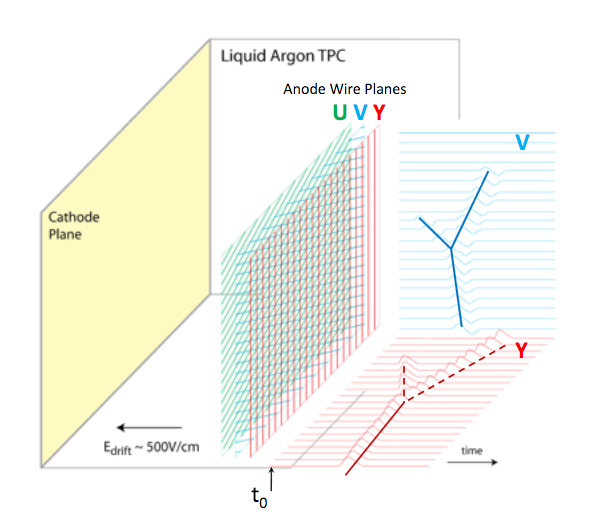
\includegraphics[width=0.4\linewidth]{Figures/detector2.png} \\
\caption{\textit{A diagram of the time projection chamber of the MicroBooNE detector \cite{lartpc}.}}\label{detector_fig}
\end{figure}

The MicroBooNE detector is currently the largest LArTPC in the United States. It consists of a rectangular time projection chamber (TPC) with dimensions 2.6 m width $\times$ 2.3 m height $\times$ 10.4 m length located 470 m away from the Booster Neutrino Beam (BNB) target. Time projection chambers, filled with a gas or liquid volume, are used to analyze particle interactions in three dimensions. The x-direction of the TPC corresponds to the drift coordinate, the y-direction is the vertical direction, and the z-direction is the direction along the beam. The amount of active liquid argon in the TPC is 89 tons, with the total cryostat containing 170 tons of liquid argon. Liquid argon is chosen to fill the volume for a variety of reasons: argon contains a high density of nucleons, which allows for a greater rate of interactions with particles within the medium; argon ionizes easily; it is transparent to itw own scintillation light; it has a high electron lifetime; and it is inexpensive.\\

Photomultiplier tubes (PMTs) and three wire planes with 3mm spacing at angles of 0, and $\pm$ 60 degrees with respect to the vertical are located in the TPC to aid with event reconstruction (Figure \ref{detector_fig}). In a neutrino interaction, a neutrino from the beam interacts with the argon and the charged outgoing child particles traverse the medium, losing energy and leaving an ionization trail. The resulting electrons drift to the anode side of the TPC, containing the wire planes, away from the negatively charged cathode plate on the opposite side. The movement of electrons induces a current in the wires, which is used to create three distinct two-dimensional views of the event. Combining these wire signals with timing information from the PMTs allows for full three-dimensional reconstruction of the event.\\


% One of the aims of MicroBooNE is to explore neutrino oscillations. For the two neutrino case, the probability that a neutrino with an initial flavor $\alpha$ will be observed as a neutrino with a different flavor $\beta$ when measured is: 

% \begin{equation}
%     P_{\alpha \rightarrow \beta}=\text{sin}^2(2\theta)\text{sin}^2(\frac{\Delta m^2 L}{4E})
% \end{equation}

% \noindent where $\theta$ is the mixing angle, $L$ is the distance from the neutrino source to the detector, $E$ is the energy of the neutrino, and $\Delta m^2$ is the neutrino squared mass difference. $\theta$ and $\Delta m^2$ are the two free parameters of interest in the above equation. The probability $P$ can be determined through a measurement of observed neutrino events compared to expected events, the distance $L$ is readily determined and constant, and $E$ can be computed from the energies of the neutrino's interaction products. 

The BNB is predominantly composed of muon neutrinos, which can undergo charge-current interactions in the TPC and produce muons. For muon tracks that are completely contained in the TPC, it is straightforward to calculate the momentum with a measurement of the length of the particle's track. Around half of muons from BNB neutrino events in {\ub} are not fully contained in the TPC, and therefore using length-based calculations for these uncontained tracks is not a possibility. The only way to compute the energy of an outgoing three-dimensional track is by means of multiple coloumb sccattering (MCS). \\

The phenomenon of multiple coulomb scattering (MCS) occurs when a charged particle enters a medium and undergoes electromagnetic scattering with the atomic nuclei. This scattering deviates the original trajectory of the particle within the material (Figure \ref{mcs_nocap_fig}). For a given energy, the scatters of a track-like particle (in terms of angular deflection relative to the track direction) form a gaussian distribution centered at zero with a and standard deviation given by the Highland formula \cite{highland}: 

\begin{equation}
	\sigma_\theta^0=\frac{13.6\  \text{MeV}}{p\beta c}z\sqrt{\frac{\ell}{X_0}}\Big[1+0.0038\text{ln}\Big(\frac{\ell}{X_0}\Big)\Big]
\end{equation}\label{highland_eqtn}

\noindent where $\beta$ is the ratio of the particle's velocity to the speed of light, $\ell$ is the distance traveled inside the material, and $X_0$ is the radiation length of the target material (taken to be a constant 14 cm in liquid argon). With the Highland formula, the momentum of a track-like particle can be determined using only the 3D reconstructed track it produces in the detector, without any calorimetric information. The method by which this is done is described in detail in Section \ref{MCS_technique_section}.

\begin{figure}[ht!]
\centering
	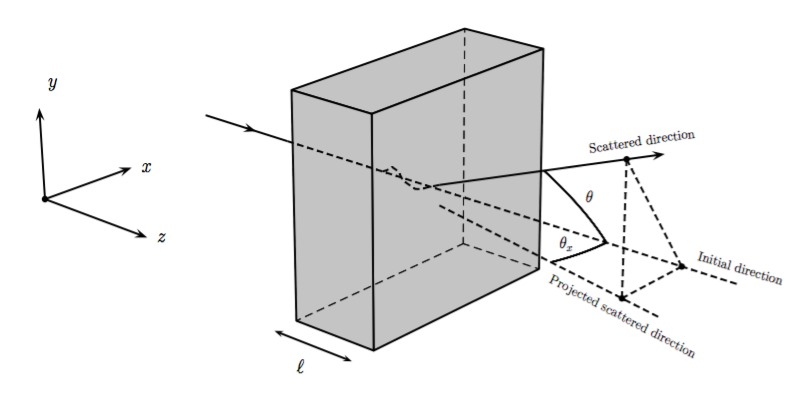
\includegraphics[width=0.5\linewidth]{Figures/mcs_nocap.png} \\
\caption{\textit{The particle's trajectory is deflected as it traverses through the material \cite{leonidas1}.}}\label{mcs_nocap_fig}
\end{figure}
\clearpage
%%%% SIGNAL SECTION %%%%
\section{MCS Implementation Using the Maximum Likelihood Method}\label{MCS_technique_section}

This section describes exactly how the phenomenon of multiple coloumb scattering is leveraged to determine the momentum of a track-like particle reconstructed in a LArTPC. In general, the approach is as follows:
\begin{enumerate}
\item The three-dimensional track is broken up into segments of configurable length.
\item The scattering angles between each consecutive segment are measured.
\item Those angles combined with the Highland formula (Equation \ref{highland_eqtn}) are used to build a likelihood that the particle has a specific momentum, taking into account energy loss in upstream segments of the track.
\item The momentum corresponding to the maximum likelihood is chosen to be the MCS computed momentum.
\end{enumerate}
Each of these steps are discussed in detail in the following subsections.\\

The idea and initial implementation of MCS using the maximum likelihood method for this analysis is credited to Leonidas Kalousis, a former member of the MicroBooNE collaboration. Further details regarding the technique can be found in his internal notes concerning both Monte Carlo simulated tracks \cite{leonidas1} and reconstructed tracks \cite{leonidas2}. Only slight modifications to this code have been made for the analysis described in this note.\\

For this analysis, a minimum start-to-end reconstructed track length of 100 cm was used.% Additionally, the relativistic limit approcimation was also used ($\beta \approx 1$ and $E \approx p$).

\subsection{Track Segmentation}\label{track_segmentation_section}
The input to the track segmentation routine is a vector of ordered three-dimensional trajectory points (x,y,z) representing the reconstructed track. The points are ordered along the direction of the track, with the first point representing the start of the track, and the last point representing the end of the track. These trajectory points can be determined in a number of ways by different track reconstruction algorithms. In general, a three-dimensional track is reconstructed by combining two-dimensional hits reconstructed from signals on the different wire planes along with timing information from the photomultiplier tubes to reconstruct the third dimension. In the case of this note, the PandoraNuPMA algorithm is used to reconstruct the track \cite{Marshall:2015rfa}.\\

Also input to the track segmentation routine is the desired segment length, which is a tunable parameter. In this note, segment lengths are generally taken to be 10 cm (based on the findings of Section \ref{SegmentLength_MCBNBRecoTrack_section}) except where otherwise explicitly stated (as in Section \ref{SegmentLength_MCBNBRecoTrack_section}). This routine begins at the start of the track, and iterates through the trajectory points in order, each time computing the straight-line distance between the first point and the current one. When a point is reached that is greater than the desired segment length, that iteration stops and the direction cosines of this segment are computed.\\

Given the subset of the three-dimensional trajectory points (x, y, z) that correspond to one ``segment" of the track, a three-dimensional linear fit is applied to the data points using the orthogonal distance regression method around the trajectory point averages for that segment. This method finds the eigenvalues and eigenvectors of the (data - average) covariance matrix and the solution is the one associated with the maximum eigenvalue.\\

At the end of this routine, a vector of length $n$ (where $n$ is the number of segments for the track) is stored containing the direction cosines at the start of each segment.


\subsection{Scattering Angle Computation}\label{scattering_angle_computation_section}
This routine within the MCS code takes as input the vector of length $n$ (where $n$ is the number of segments for the track) containing the direction cosines at the start of each segment. In general, the algorithm iterates over consecutive pairs of segments (the segmentation routine is described in Section \ref{track_segmentation_section}) and computes angular scatters between each, and stores them for later use by a future subroutine. This code is more complicated than just taking the dot product between consecutive direction cosines to find the total angular scatter between segments because the Highland formula is derived from scattering independently in the two directions orthogonal to the direction of the track. For this reason, this subroutine performs a coordinate transformation for each pair of segments such that the ``z'' direction (which, in detector coordinates is just the beam direction) is rotated to be along the direction of the first two segments. With the ``z'' direction as such, ``x'' and ``y'' directions are chosen such that all of ``x'', ``y'', and ``z'' are mutually orthogonal. Note that at this point, all of ``x'', ``y'', and ``z'' are different than the similarly named detector coordinates. The scattering angle both in the ``x'' and ``y'' planes are then computed for each consecutive pairs of segments. After this routine, a vector of length $2n$ is stored containing the scattering angles in the ``x'' plane as well as in the ``y'' plane. These scattering angles are what are input into the maximum likelihood routine to determine track momentum.


\subsection{Maximum Likelihood Theory}\label{likelihood_theory_section}

The normal probability distribution for a variable with a gaussian error sigma is given by:
\begin{equation}
f_X(\Delta\theta_j) = (2\pi\sigma_0^2)^{-\frac{1}{2}}exp(-\frac{1}{2}\frac{(\Delta\theta_j-\mu_0)^2}{\sigma_0^2})
\end{equation}

Here, each $\Delta\theta_j$ corresponds to a $\Delta\theta$ measurement between one pair of segments in a track either in the rotated-coordinates ``x'' or ``y'' plane, $\mu_0$ is assumed to be zero, and $\sigma_\theta^0$ is the RMS angular deflection computed by the modified Highland formula (Equation \ref{modified_highland_eqtn}), which is a function of both the momentum and the length of that segment. Since energy is lost between segments, $\sigma_\theta^0$ is different for each angular measurement along the track so we replace $\sigma_\theta^0$ with $\sigma_\theta^j$, where $j$ is an index representative of the segment. \newline

To get the likelihood, one takes the product of $f_X(\Delta\theta_j)$ over all the $\Delta\theta_j$ segment-to-segment scatters along the track. Since the product of exponentials is just an exponential with the sum of the arguments, this product becomes
\begin{equation}
L(\mu;(\sigma_\theta^1)^2,...,(\sigma_\theta^n)^2;\Delta\theta_1,...,\Delta\theta_n) = \prod_{j=1}^{n}f_X(\Delta\theta_j,\mu,(\sigma_\theta^j)^2) = (2\pi)^\frac{-n}{2}\times\prod_{j=1}^{n}(\sigma_\theta^j)^{-1} \times exp(-\frac{1}{2}\sum_{j=1}^{n}\frac{(\Delta\theta_j-\mu_0)^2}{(\sigma_\theta^j)^2})
\end{equation}

In practice, rather than maximizing likelihood it is often more computationally convenient to instead minimize the negative log likelihood. Taking the natural logarithm of the likelihood $L$ gives an expression that is related to a $\chi^2$
\begin{equation}\label{leo_llhd_eqtn}
l(\mu;(\sigma_\theta^1)^2,...,(\sigma_\theta^n)^2;\Delta\theta_1,...,\Delta\theta_n) = ln(L) = -\frac{n}{2}ln(2\pi) - \sum_{j=1}^{n}ln(\sigma_\theta^j) - \frac{1}{2}\sum_{j=1}^{n}\frac{(\Delta\theta_j-\mu)^2}{(\sigma_\theta^j)^2}
\end{equation}

The negative log likelihood for one specific segment's angular scatter $\Delta\theta_j$ given an expected scattering RMS $\sigma_\theta^j$ is given by the following equation
\begin{equation}\label{negative_llh_eqtn}
-l(\mu, \sigma_\theta^j, \Delta\theta_j) = \frac{1}{2}ln(2\pi) + ln(\sigma_\theta^j) + \frac{1}{2}\frac{(\Delta\theta_j-\mu)^2}{(\sigma_\theta^j)^2}
\end{equation}

In general, Equation \ref{negative_llh_eqtn} is evaluated for each segment in a track given a postulated full track momentum, and the sum of these terms is used to determine the likelihood that the postulated track momentum is correct for that track.


\subsection{Maximum Likelihood Implementation}\label{maximum_likelihood_section}

Given a set of angular deflections in the ``x'' and ``y'' planes for each segment as described in Section \ref{scattering_angle_computation_section}, a modified version of the Highland formula (Equation \ref{modified_highland_eqtn}) is used along with a maximum likelihood method to determine the momentum of the track. 

\begin{equation}\label{modified_highland_eqtn}
\sigma_{\theta}^{RMS} = \sqrt{ (\sigma_\theta^0)^2 + (\sigma_\theta^{res})^2} = \sqrt{ (\frac{13.6\  \text{MeV}}{p\beta c}z\sqrt{\frac{\ell}{X_0}}\Big[1+0.0038\text{ln}\Big(\frac{\ell}{X_0}\Big)\Big])^2 + (\sigma_\theta^{res})^2 }
\end{equation}
where the formula is ``modified'' from the original Highland formula (Equation \ref{highland_eqtn}) in that it includes a detector-inherent angular resolution term $\sigma_\theta^{res}$ which is given a fixed value of 2 mrad in this analysis as described in Section \ref{ResolutionStudy_MCBNBRecoTrack_section}\cite{leonidas2}.\\

In general, this routine does a raster scan over postulated track energies in steps of 1 MeV from a minimum of the full track range-based momentum up to a maximum of 7.5 GeV. Starting with the range-based momentum as a minimum is valid because the range-based momentum is known to be an accurate predictor of momentum for contained tracks (see Section \ref{Range_Energy_Validation_section}) and is therefore an acceptable minimum both for contained and for exiting tracks. Ending at 7.5 GeV as a maximum momentum is valid because given the BNB spectrum, no neutrino-induced tracks above that momentum are expected in {\ub}.\\

Given a postulated full track momentum, the full track energy $E_t$ is computed from the usual energy momentum relation,
\begin{equation}\label{energy_momentum_relation_eqtn}
E^2 = p^2 + m^2
\end{equation}
 and the maximum likelihood algorithm iterates over angular scatters for each segment, with two $\Delta\theta_j$ values for each segment (corresponding to the ``x'' and ``y'' scattering planes). The energy of the $j$th segment is given by
\begin{equation}\label{segment_E_equation}
E_{j} = E_t - k_{cal}*N_{upstream}*l_{seg}
\end{equation}
where $k_{cal}$ is the minimally ionizing energy constant given to be $2.105 \frac{MeV}{cm}$ in liquid argon\cite{MIPenergysource}, $N_{upstream}$ is the number of segments upstream of this particular segment, and $l_{seg}$ is the segmentation length. This definition of $E_j$ therefore takes into account energy loss along the track, and can never be negative given the range of possible $E_t$ values described previously. This value of segment energy is used to predict the RMS angular scatter for that segment ($\sigma_\theta^{RMS}$) by way of a modified version of the modified Highland formula, Equation \ref{modified_highland_eqtn}. Still assuming the mean angular scatter, $\mu$, is zero, Equation \ref{negative_llh_eqtn} is evaluated for each segment and all evaluations are summed to compute a total summed negative log likelihood for that postulated track energy, $E_t$.\\

After the raster scan over postulated track momenta is complete, the one with the smallest summed negative log likelihood is chosen to be the final MCS computed momentum for the track.













%Initial contents of technique.tex below, commented out as per request. -Polina

%\begin{enumerate}
%\item this will be a detailed description of exactly how the algorithm works. it will start with a copy/paste of polina's section 1B then i will add details.
%\item details that need to be added include a description of all of the knobs that can be turned in the MCS code: the resolution term, the step size in the energy raster scan, the segment length, and whether to use x- scatters, y- scatters, or both.
%\item possible plot: the highland formula RMS versus segment energy so people can visualize how much more "straight" a 1 GeV muon segment is than a 500 MeV muon segment, etc... some explanation that a muon loses MIP energy as it traverses LAr so scattering gets more and more, this is taken into account in our method
%\item discussion of how our method compares to icarus's (cite their paper)
%\end{enumerate}
%
%\begin{figure}
%\centering
%\mbox{
%	\subfigure[\textit{sample figure left}]
%	{
\includegraphics[width=25mm]{Figures/FILLER.png}}
%	\quad
%	\subfigure[\textit{sample figure right}]
%	{
\includegraphics[width=25mm]{Figures/FILLER.png}}
%	}
%\caption{\textit{THIS IS A SAMPLE FIGURE}}
%\label{sample_fig}
%\end{figure}





\clearpage
\section{Re-Tuning the Highland Formula for Argon}\label{highland_retuning_section}
The Highland formula as given in the 1990 paper by Lynch and Dahl\cite{highland-lynch-dahl} is as follows:
\begin{equation}
	\sigma_o=\frac{13.6\  \text{MeV}}{p\beta c}z\sqrt{\frac{\ell}{X_0}}\Big[1+0.0038\text{ln}\Big(\frac{\ell}{X_0}\Big)\Big]
\end{equation}

The constants in the formula ($13.6$ and $0.0038$) were determined using a fit to simulated particles: ``the subroutine GMOLS that is in the GEANT Monte Carlo program to generate $10^6$ scatters of singly charged heavy particles for 14 different elements and 7 different thicknesses ranging from $10^{-4}$ radiation lengths to 100 radiation lengths.'' All of their simulated particles were relativistic, with $\beta=1$. The materials in which they studied scattering ranged from hydrogen (with Z=1) to uranium (with Z=92). Given that the constants in the formula were determined from a fit to a widge range of Z with a wide range of material thicknesses (analogous to segmentation length in this analysis), there is reason to believe that these constants should differ for scattering in liquid argon with segmentation length on the order of $X_o$. There is also reason to believe that these constants might change for partices with $\beta < 1$, which is the case for segments of contained muons within roughly a meter of their stopping point.\\

In order to re-tune these constants to liquid argon, a large sample of muons were simulated and their true energy depositions ({\sc MCTracks}) were used in a fit. {\sc MCTracks} are described in detail in Section \ref{MCTrack_section}. The sample of muon {\sc MCTracks} used is described in Section \ref{MCBNBMCTrack_eventselection_section}. These {\sc MCTracks} were divided into 14 cm segments as described in Section \ref{track_segmentation_section} and their angular scatters in the $x'$ and $y'$ directions were computed as described in Section \ref{scattering_angle_computation_section}. The reason for using specifically 14 cm segments is that 14 cm is also the radiation length in liquid argon, so the Highland equation simplifies greatly:

\begin{equation}\label{highland_simplified}
	\sigma_o=\frac{13.6\  \text{MeV}}{p\beta c}
\end{equation}

Equation \ref{highland_simplified} was used to compute the RMS scattering angle for each segment of these {\sc MCTracks}, using the true momentum of the muon at the start of each segment. Note that this equation does not include the detector-inherent angular resolution term $\sigma_o^{res}$ quoted in Equation \ref{modified_highland_eqtn} because {\sc MCTracks} have perfect resolution. If Equation \ref{highland_simplified} is correct, a histogram of angular scatter divided by $\sigma_o$ should be gaussian with a width of unity\footnote{Note that Lynch and Dahl recommend fitting only the central portion (E.G. 98\%) of this distribution to mitigate the effect of large angle (non-gaussian) scatters which are not well described by the Highland formula, but in this analysis the entire distribution is fit as the entire distribution is what is used in the algorithm itself.}. This distribution is shown in Figure \ref{retune_highland_fig1}. The width of this distribution (about 0.88) is less than 1. The 13.6 constant in Equation \ref{highland_simplified} was varied gradually and it was found that by decreasing the constant, this distribution is widened, and a constant of about 12.0 will bring the width to unity. This distribution is shown in Figure \ref{retune_highland_fig2}.\\ 



\begin{figure}
\centering
\mbox{
	\subfigure[\textit{Equation \ref{highland_simplified} is used to compute the denominator. Note the fitted gaussian width is less than 1.}\label{retune_highland_fig1}]
	{\includegraphics[width=75mm]{Figures/{contained_MCTracks_13.6_gaussian}.png}}
	\quad
	\subfigure[\textit{Equation \ref{highland_simplified} (with 12.0 as the constant in place of 13.6) is used to compute the denominator. Note the fitted gaussian width is 1.}\label{retune_highland_fig2}]
	{\includegraphics[width=75mm]{Figures/{contained_MCTracks_12.0_gaussian}.png}}
	}
\caption{\textit{14 cm segment angular deviations divided by expected Highland RMS for the contained single muon {\sc MCTrack} sample described in Section \ref{MCBNBMCTrack_eventselection_section} when Equation \ref{highland_simplified} is used (along with the true segment momentum) to compute the denominator.}}
\end{figure}


However, many of the segments included in Figure \ref{retune_highland_fig2} are non-relativistic, as the sample of {\sc MCTracks} studied correspond to stopping muons. Selecting only highly relativistic segments (with true momentum above 1 GeV) leads one to determine the constant should be closer to 11.0. In order to account for the the apparent $\beta$ (or $p$) dependence of this constant, the {\sc MCTrack} segments were grouped in bins of true momentum and a constant was fit for each. The fitted constant value as a function of true momentum is shown in Figure \ref{retune_highland_fig3}.\\

\begin{figure}[ht!]
\begin{center}
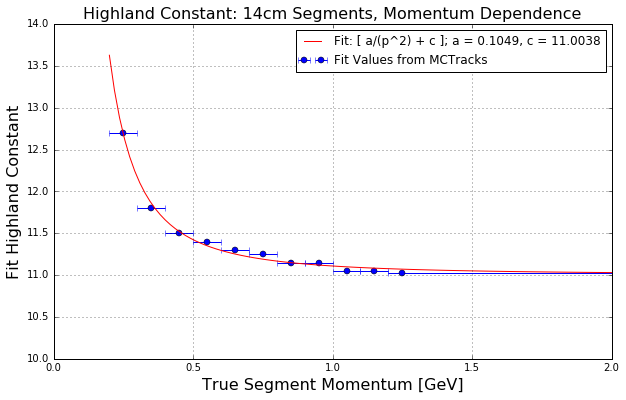
\includegraphics[width=100mm]{Figures/highland_constant_optimization_momentumdependent.png}
\end{center}
\caption{\textit{Fitted Highland constant as a function of true segment momentum for 14 cm segments of {\sc MCTracks}. Blue x- error bars indicate true momentum bin width with data points drawn at the center of each bin, except for the highest momentum bin which includes the segment momentum tail that extends beyond the limit of the plot, up to 6 GeV. Shown in red is a fit to these data points with functional form $\frac{a}{p^2} + c$, with converged values for floating constants $a$ and $c$ shown in the legend.}}
\label{retune_highland_fig3}
\end{figure}

Note that the highest momentum point in Figure \ref{retune_highland_fig3} represents a bin which extends from 1.10 GeV to 6 GeV, capturing the entire high momentum ($\beta = 1$) tail of the true {\sc MCTrack} segment momentum distribution. It can be seen that the fitted value asymptotically approaches a constant at higher momentum (where $\beta = 1$) of about 11.0. The value increases in the momentum region where $\beta < 1$. Shown in red is a fit to these data points with functional form $\frac{a}{p^2} + c$, with converged values for floating constants $a$ and $c$ shown in the legend. This functional form was chosen because it fit the data well, and asymptotically approaches a constant value when $\beta$ approaches 1. The fitted values for $a$ and $c$ are 0.1049 and 11.0038 respectively. This function will henceforth be referred to as $\kappa(p)$:
\begin{equation}
\kappa(p) = \frac{0.1049}{p^2} + 11.0038
\end{equation}\label{kappa_equation}

In this analysis, $\kappa(p)$ is used as a replacement for the 13.6 constant in the Highland formula. Note that with 14 cm segments, the smallest segment momentum the algorithm plugs into Equation \ref{kappa_equation} corresponds to the left-most value of the fit drawn, a Highland constant of about 13.7, so the rapid increase of $\kappa(p)$ for small values of $p$ is not an issue. The effect of replacing 13.6 with $\kappa(p)$ in the Highland equation is to reduce a systematic bias that was present in the algorithm, in which the algorithm overestimated the true momentum of muons. To visualize the Highland formula for 14 cm segments both before and after the $\kappa(p)$ replacement, see Figure \ref{retune_highland_fig4}. It is recommended that future LArTPC experiments use this parameterization of the Highland formula, or at the very least conduct their own studies fit for the 13.6 constant in the Highland formula, which clearly is not the correct value for liquid argon specifically.\\

\begin{figure}[ht!]
\begin{center}
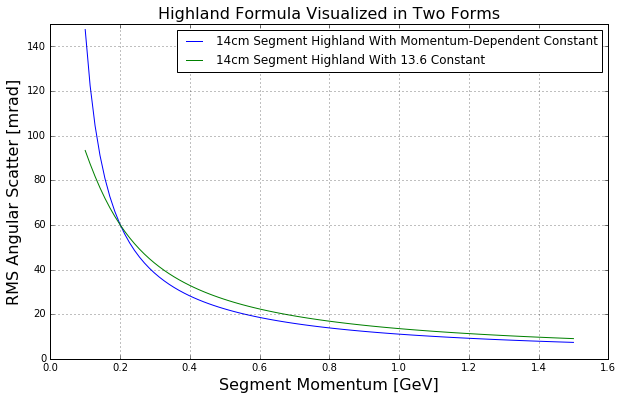
\includegraphics[width=100mm]{Figures/highland_formula_visualized_twoforms.png}
\end{center}
\caption{\textit{The Highland scattering RMS $\sigma_o$ for 14 cm segment lengths and 0 detector-inherent angular resolution as a function of true momentum before and after retuning. In green is shown Equation \ref{highland_simplified} (using 13.6 constant) and in blue is the same equation replacing 13.6 with $\kappa(p)$.}}
\label{retune_highland_fig4}
\end{figure}



The form of the Highland equation used in this analysis is therefore given by Equation \ref{modified_highland_eqtn}, with $\kappa(p)$ given by Equation \ref{kappa_equation}, noting that with segmentation length $\ell = X_0 = 14 cm$ the formula simplifies greatly. For the sake of readability, Equation \ref{modified_highland_eqtn} is rewritten here:
\begin{equation}
\sigma_{o}^{RMS} = \sqrt{ (\sigma_o)^2 + (\sigma_o^{res})^2} = \sqrt{ (\frac{\kappa(p)}{p\beta c}z\sqrt{\frac{\ell}{X_0}}\Big[1+0.0038\text{ln}\Big(\frac{\ell}{X_0}\Big)\Big])^2 + (\sigma_o^{res})^2 }
\end{equation}


% DEPRICATED
%% 
\section{MCS Performance on Simulated Single Muons}\label{singlemuon_MC_section}

% Executive summary
In this section, MCS performance is studied on a sample of simulated, fully contained, single muons in {\ub}. It is demonstrated that the range-based energy of a track agrees with the true energy with negligible bias and with a resolution of better than 5\%. The MCS performance on single {\sc MCTracks} is shown to be comparable to that on single reconstructed PandoraNuPMA tracks when the track is well reconstructed, with a minimal bias and a resolution that varies between 5 and 20\%, performing better for higher energy (longer) tracks. Additionally, the scattering angle of track segments for a given energy is shown to be gaussian, in line with the Highland formula prediction both for {\sc MCTracks} and reconstructed tracks.


\subsection{Input Sample}\label{SingleMu_Input_Sample_section}
In order to study MCS performance in the most straightforward way, a sample of simulated single muons is used. This sample was generated in the {\ub} MCC7 production under the SAM definition ``prod\_muminus\_0-2.0GeV\_isotropic\_uboone\_mcc7\_reco2''. This sample consists of 19,500 single muons generated at a random location within the {\ub} TPC, with random direction. The energy spectrum of this sample is flat between 0 to 2 GeV kinetic energy of the muons. It is worth noting that the MCC7 simulation includes broken wires by masking specific channels on some planes in an attempt to better match real detector conditions (XXX reference about MCC7?).\\

This section of the technote will include studies from this single muon sample, both with {\sc MCTracks} (described in Section \ref{MCTrack_section}) and with reconstructed tracks (described in Section \ref{RecoTrack_section}).

\subsection{Fiducial Volume Definition}\label{fidvol_section}
The {\ub} TPC has active volume dimensions of 2.3 m width $\times$ 2.6 m height $\times$ 10.4 m length. For this analysis, a smaller ``fiducial volume'' is defined and referenced throughout this note (for example, in many cases reconstructed tracks are required to be fully contained within the fiducial volume). For reference, the fiducial volume definition used throughout this note is the full TPC volume reduced in by 20 cm from both the cathode plane and the anode wire planes, shifted in 26.5 cm in from both the top and bottom walls of the TPC, shifted in 20 cm from the beam-upstream wall of the TPC, and shifted in 36.8 cm from the downstream wall of the TPC. The reason for this choice of fiducial volume is that it reduces contamination from ``edge effects'' that occur near the walls of the TPC, like electric field distortions and space-charge effects. While the TPC has a total active volume of 62.6 $m^3$, the fiducial volume used in this analysis has a volume of 38.7 $m^3$ or roughly 62\% of the total TPC active volume.


%%%%%%%%%%%%%%%%%%%%%%%%%%%%%%%%%%%%%%%%%%%%%%%%%%%%%%%%%%%%%%%%%%%%%%%%%%%%%%%%%%%%%
\subsection{Performance with \sc{MCTracks}}


\subsubsection{MCTrack Description}\label{MCTrack_section}
{\sc MCTrack} objects are made from the output of {\sc geant}4, and are created from {\sc geant}4 energy depositions in the detector. {\sc geant}4 outputs 3D energy depositions in the detector, along with truth information about which parent particles deposited this energy. {\sc MCTracks} are 3D objects which are formed by grouping the energy depositions based on parent particles. Whether a particle in {\sc geant}4 is turned into an {\sc MCTrack} or an {\sc MCShower} (not discussed in this note) is based on truth PDG (for example, muons, protons, and pions always form {\sc MCTracks}).\\

Each {\sc MCTrack} is itself a vector of 3D trajectory points, which are ordered to match the direction of the particle that deposited the energy. Trajectory points are only formed for energy depositions inside of the TPC volume. In general, long {\sc MCTrack}s will have steps separated by up to several centimeters. Each step in an {\sc MCTrack} holds the following information used in this analysis: 3D position, and true energy at that point. Only information within the realm of reconstructable quantities is used in this analysis, with the exception of true energy (which is used for example to quantify a reconstructed energy resolution).\\

Since the output of a nominal reconstruction chain (going through hit finding, clustering, matching across planes, etc.) are 3D tracks, {\sc MCTracks} can be studied in an analysis in the exact same way as a reconstructed track would be. {\sc MCTracks} can be thought of as perfectly reconstructed tracks, where each trajectory point along the track is a true 3D energy deposition inside of the {\ub} TPC.\\

Since {\sc MCTracks} are formed from true 3D energy depositions and not from wire signals on drift electrons, {\sc MCTracks} are insensitive to broken wires, noise, and other simulated detector effects.

\subsubsection{MCTrack Selection}\label{MCTrack_Selection_section}
For analysis on single muon {\sc MCTracks}, the input sample is the one described in Section \ref{SingleMu_Input_Sample_section}. From that sample, the following requirements are placed for event selection:
\begin{enumerate}
	\item There is exactly one {\sc MCTrack} in the event.
	\item The {\sc MCTrack} is longer than one meter in start-to-end length.
	\item The {\sc MCTrack} is fully contained within the fiducial volume (defined in Section \ref{fidvol_section}).
	\item The {\sc MCTrack} does not decay in flight.
\end{enumerate}
After these selection requirements are placed, the intial sample of 19,500 muons is reduced to 623 which are used for analysis.

\subsubsection{Range Energy Validation}\label{Range_Energy_Validation_section}
With this sample of {\sc MCTracks}, it is possible to quantify MCS energy resolution as a function of true energy. However, in actual {\ub} data there is obviously no true energy with which to compare. The additional energy handle that is used in data for contained tracks is range-based energy. The stopping power of muons in liquid argon is well described by the particle data group\cite{PDG_spline_table}. By using a linear interpolation between points in the cited PDG stopping power table, the start-to-end length of a track can be used to reconstruct the muon's total energy with good accuracy. Figure \ref{true_range_energy_MCTrack_fig} shows a comparison of range energy to true energy for this sample. \\

In order to compute a bias and a resolution, Figure \ref{true_range_energy_MCTrack_fig} is sliced in bins of true muon energy and a histogram of the fractional energy difference ($\frac{E_{range} - E_{true}}{E_{true}}$) is created for each bin. This distribution is shown for three representative bins in Figure \ref{true_range_bias_resolution_MCTrack_slices_fig}. The mean of each distribution is used to compute a bias a function of true energy, while the standard deviation of each distribution is used to compute a resolution. Figure \ref{true_range_bias_resolution_MCTrack_fig} shows the bias and resolution for the range-based energy reconstruction method. It can be seen that the bias is negligible and the resolution for this method of energy reconstruction is on the order of 2-4\%. Based on this figure, it is clear that range-based energy is a good handle on the true energy of a reconstructed muon track in {\ub} data, assuming that track starts and ends near the true start and end of the muon.

\begin{figure}[h!]
\begin{center}
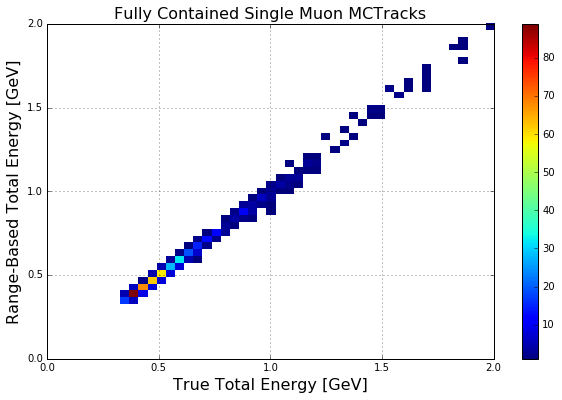
\includegraphics[width=100mm]{Figures/true_range_comparison_MCTracks.png}
\end{center}
\caption{\textit{Range based energy versus true energy for the single muon {\sc MCTrack} sample described in Section \ref{MCTrack_Selection_section}.}}
\label{true_range_energy_MCTrack_fig}
\end{figure}

\begin{figure}
\centering
\mbox{
	\subfigure[\textit{Fractional energy difference between 0.35 and 0.53 GeV true energy.}]
	{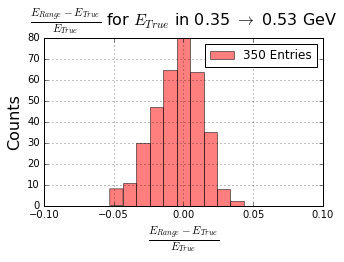
\includegraphics[width=50mm]{Figures/true_range_resolution_MCTracks_slice1.png}}
	\quad
	\subfigure[\textit{Fractional energy difference between 0.90 and 1.08 GeV true energy.}]
	{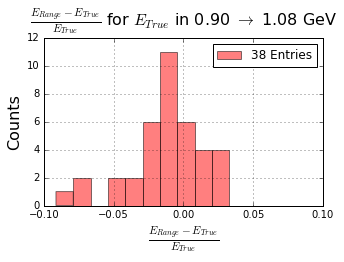
\includegraphics[width=50mm]{Figures/true_range_resolution_MCTracks_slice2.png}}
	\quad
	\subfigure[\textit{Fractional energy difference between 1.45 and 1.63 GeV true energy.}]
	{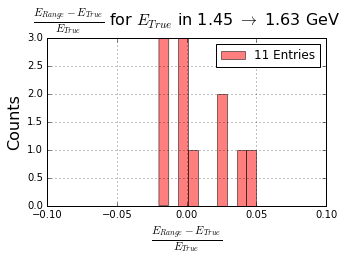
\includegraphics[width=50mm]{Figures/true_range_resolution_MCTracks_slice3.png}}
	}
\caption{\textit{Fractional energy difference for a few representative bins of true energy derived from Figure \ref{true_range_energy_MCTrack_fig}.}}
\label{true_range_bias_resolution_MCTrack_slices_fig}
\end{figure}




\begin{figure}
\centering
\mbox{
	\subfigure[\textit{Range energy bias as a function of true energy.}]
	{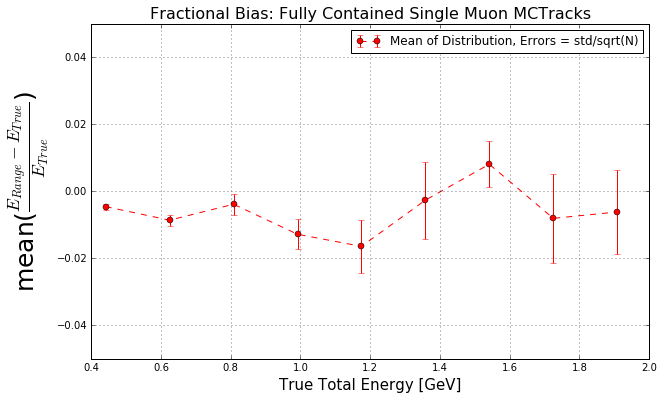
\includegraphics[width=75mm]{Figures/true_range_bias_MCTracks.png}}
	\quad
	\subfigure[\textit{Range energy resolution as a function of true energy.}]
	{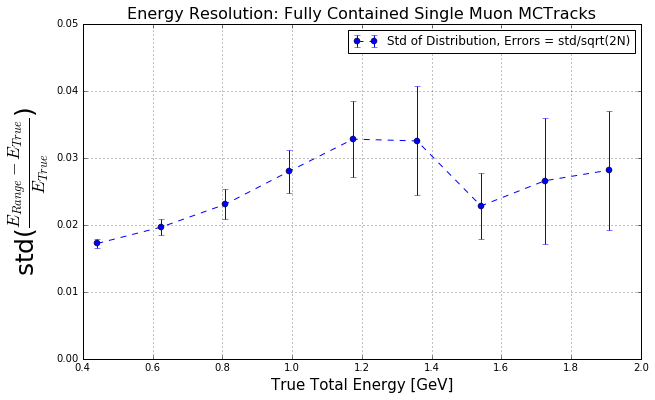
\includegraphics[width=75mm]{Figures/true_range_resolution_MCTracks.png}}
	}
\caption{\textit{Range energy and true energy bias and resolution for the single muon {\sc MCTrack} sample described in Section \ref{MCTrack_Selection_section}.}}
\label{true_range_bias_resolution_MCTrack_fig}
\end{figure}




\subsubsection{MCS Energy Validation}\label{MCS_Energy_Validation_MCTrack_section}
For this sample of {\sc MCTracks}, only the trajectory points of each {\sc MCTrack} are used as input to the MCS code, described in Section \ref{MCS_technique_section}. The resulting MCS energy versus range-based energy can be seen in Figure \ref{MCS_range_energy_MCTrack_fig}. Range energy is used here instead of true energy in order to make this plot more directly comparable with the same analysis on data where true energy is not accessible\footnote{It is acceptable to use range energy based on Figure \ref{true_range_bias_resolution_MCTrack_fig}.}. In order to compute a bias and a resolution, Figure \ref{MCS_range_energy_MCTrack_fig} is sliced in bins of range energy and a histogram of the fractional energy difference ($\frac{E_{MCS} - E_{range}}{E_{range}}$) is created for each bin. This distribution is shown for three representative bins in Figure \ref{MCS_range_bias_resolution_MCTrack_slices_fig}. The mean of each distribution is used to compute a bias a function of range energy, while the standard deviation of each distribution is used to compute a resolution. The bias and resolution for this energy reconstruction method shown in Figure \ref{MCS_range_bias_resolution_MCTrack_fig}. This figure indicates a bias in the MCS energy resolution on the order of a few percent, with a resolution that decreases from about 18\% for contained {\sc MCTracks} with true total energy around 0.5 GeV (which corresponds to a length of about 1.7 meters) to below 10\% for contained {\sc MCTracks} with true total energy greater than 0.8 GeV (which corresponds to a length of about 3.1 meters).


\begin{figure}[h!]
\begin{center}
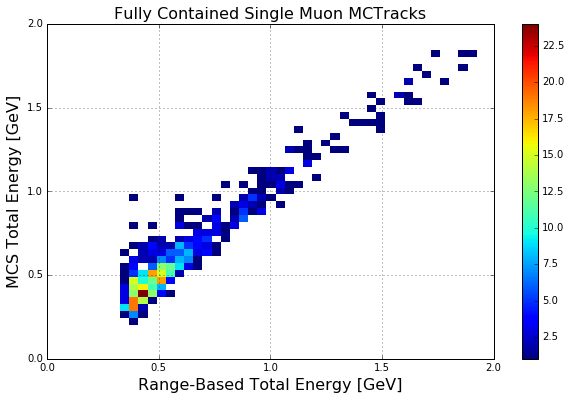
\includegraphics[width=100mm]{Figures/MCS_range_comparison_MCTracks.png}
\end{center}
\caption{\textit{MCS computed energy versus range energy for the single muon {\sc MCTrack} sample described in Section \ref{MCTrack_Selection_section}.}}
\label{MCS_range_energy_MCTrack_fig}
\end{figure}

\begin{figure}
\centering
\mbox{
	\subfigure[\textit{Fractional energy difference between 0.35 and 0.53 GeV range energy.}]
	{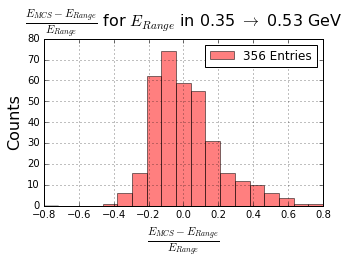
\includegraphics[width=50mm]{Figures/MCS_range_resolution_MCTracks_slice1.png}}
	\quad
	\subfigure[\textit{Fractional energy difference between 0.90 and 1.08 GeV range energy.}]
	{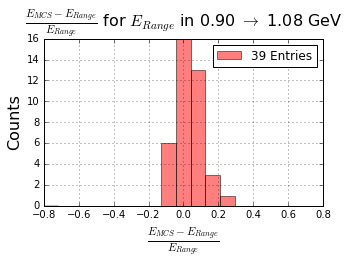
\includegraphics[width=50mm]{Figures/MCS_range_resolution_MCTracks_slice2.png}}
	\quad
	\subfigure[\textit{Fractional energy difference between 1.45 and 1.63 GeV range energy.}]
	{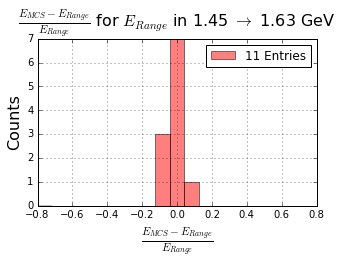
\includegraphics[width=50mm]{Figures/MCS_range_resolution_MCTracks_slice3.png}}
	}
\caption{\textit{Fractional energy difference for a few representative bins of range energy derived from Figure \ref{MCS_range_energy_MCTrack_fig}.}}
\label{MCS_range_bias_resolution_MCTrack_slices_fig}
\end{figure}


\begin{figure}
\centering
\mbox{
	\subfigure[\textit{MCS energy bias as a function of range energy.}]
	{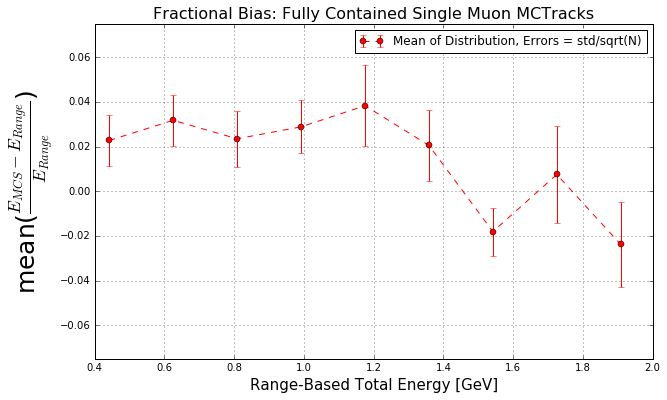
\includegraphics[width=75mm]{Figures/MCS_range_bias_MCTracks.png}}
	\quad
	\subfigure[\textit{MCS energy resolution as a function of range energy.}]
	{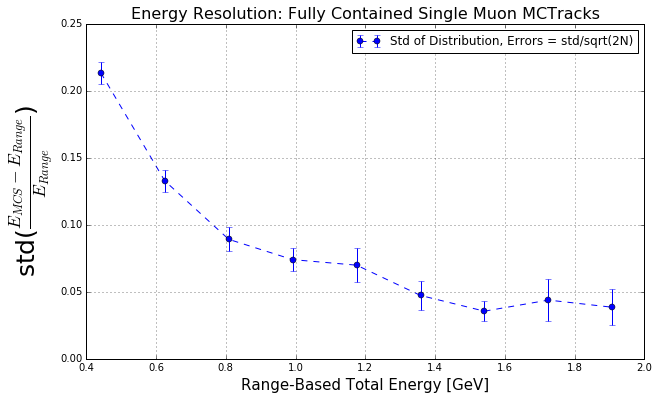
\includegraphics[width=75mm]{Figures/MCS_range_resolution_MCTracks.png}}
	}
\caption{\textit{MCS energy bias and resolution as a function of range energy for the single muon {\sc MCTrack} sample described in Section \ref{MCTrack_Selection_section}.}}
\label{MCS_range_bias_resolution_MCTrack_fig}
\end{figure}



\subsubsection{Highland Validation}\label{Highland_Validation_MCTrack_section}
For a given track segment energy and length, 98\% of the angular scatter deviations should be gaussian with an RMS described by the Highland equation (Equation \ref{highland_eqtn}), while the remaining 2\% are larger angle Rutherford scatters [XXX source]. Therefore, a histogram of track segment angular deviations divided by the RMS predicted by the Highland equation should be gaussian with a width of unity. In this section, we validate this claim.\\

For each 20cm segment of each {\sc MCTrack} in this single muon sample, the energy of the muon at the start of that segment is estimated by taking the computed MCS energy and subtracting out energy lost in the track upstream of the start of this segment, assuming the track was minimally ionizing (depositing 2.2 MeV per centimeter of track) as described in Equation \ref{segment_E_equation} where $E_t$ is the computed MCS energy of the full track. The segment energy, along with the segment length, is converted into an expected RMS angular deviation by way of Equation \ref{highland_eqtn}. For each consecutive pair of segments, the angular scatter in milliradians divided by the Highland expected RMS in millradians is an entry in the histogram shown in Figure \ref{Highland_validation_MCTracks_fig}. From this figure we can see that the Highland formula is valid for {\sc MCTracks}, as the gaussian fit agrees well with the underlying histogram.

\begin{figure}[h!]
\begin{center}
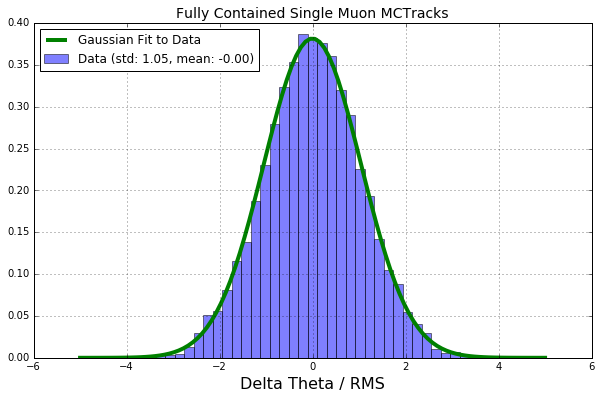
\includegraphics[width=100mm]{Figures/Highland_validation_MCTracks.png}
\end{center}
\caption{\textit{20cm segment angular deviations divided by expected Highland RMS for the single muon {\sc MCTrack} sample described in Section \ref{MCTrack_Selection_section}.}}
\label{Highland_validation_MCTracks_fig}
\end{figure}













%%%%%%%%%%%%%%%%%%%%%%%%%%%%%%%%%%%%%%%%%%%%%%%%%%%%%%%%%%%%%%%%%%%%%%%%%%%%%%%%%%%%%

\subsection{Performance with Reconstructed Tracks}
\subsubsection{Reconstructed Track Description}\label{RecoTrack_section}
XXX this section has description of PandoraNuPMA tracks, cite pandora reference rather than lengthy description.

\subsubsection{Reconstructed Track Selection}\label{RecoTrack_Selection_section}
For analysis on single muon reconstructed tracks, the input sample is the one described in Section \ref{SingleMu_Input_Sample_section}. From that sample, the requirements described in Section \ref{MCTrack_Selection_section} are first placed on the sample. Then, the following additional requirements are placed for event selection:
\begin{enumerate}
	\item There is exactly one reconstructed track in the event.
	\item The reconstructed track is longer than one meter in start-to-end length.
	\item The reconstructed track is fully contained within the fiducial volume (defined in Section \ref{fidvol_section}).
	\item The start of the reconstructed track is within 3 cm of the start of the {\sc MCTrack}, and the end of the reconstructed track is within 3c m of the end of the {\sc MCTrack} (or vice-versa).
\end{enumerate}
The last selection criteria is the one most worth noting; it ensures that the track is well reconstructed and not broken or truncated. The purpose the ``vice-versa'' clause in the last selection criteria is to take into account tracks that are well reconstructed in terms of position, but are flipped in direction. In the case of reverse-oriented tracks, the reconstructed track is flipped to have the correct direction before proceeding with the analysis. The application of these track selection cuts reduces the sample down to 307 reconstructed single muon tracks, which are used in this analysis.



\subsubsection{MCS Energy Validation}\label{MCS_Energy_Validation_RecoTrack_section}
For this sample of reconstructed tracks, only the trajectory points of each reconstructed track are used as input to the MCS code, described in Section \ref{MCS_technique_section}. The resulting MCS energy versus range-based energy can be seen in Figure \ref{MCS_range_energy_RecoTrack_fig}. In order to compute a bias and a resolution, Figure \ref{MCS_range_energy_RecoTrack_fig} is sliced in bins of range energy and a histogram of the fractional energy difference ($\frac{E_{MCS} - E_{range}}{E_{range}}$) is created for each bin. This distribution is shown for three representative bins in Figure \ref{MCS_range_bias_resolution_RecoTrack_slices_fig}. The mean of each distribution is used to compute a bias a function of range, while the standard deviation of each distribution is used to compute a resolution. The bias and resolution for this energy reconstruction method shown in Figure \ref{MCS_range_bias_resolution_RecoTrack_fig}. This figure indicates a bias in the MCS energy resolution on the order of a few percent, with a resolution that decreases from about 18\% for contained reconstructed tracks with range energy around 0.5 GeV (which corresponds to a length of about 1.7 meters) to below 10\% for contained reconstructed tracks with range energy greater than 0.8 GeV (which corresponds to a length of about 3.1 meters). This agrees very well with the same resolution and boas plots made for {\sc MCTracks} (Figure \ref{MCS_range_bias_resolution_MCTrack_fig}).


\begin{figure}[h!]
\begin{center}
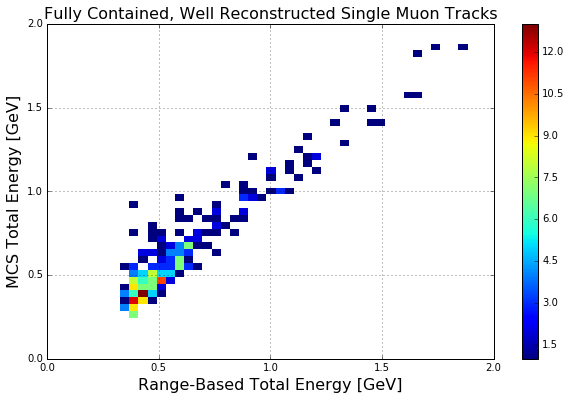
\includegraphics[width=100mm]{Figures/MCS_range_comparison_RecoTracks.png}
\end{center}
\caption{\textit{MCS computed energy versus range energy for the single muon reconstructed track sample described in Section \ref{RecoTrack_Selection_section}.}}
\label{MCS_range_energy_RecoTrack_fig}
\end{figure}

\begin{figure}
\centering
\mbox{
	\subfigure[\textit{Fractional energy difference between 0.35 and 0.53 GeV range energy.}]
	{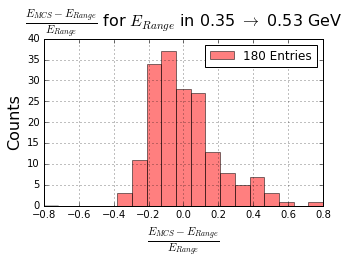
\includegraphics[width=50mm]{Figures/MCS_range_resolution_RecoTracks_slice1.png}}
	\quad
	\subfigure[\textit{Fractional energy difference between 0.90 and 1.08 GeV range energy.}]
	{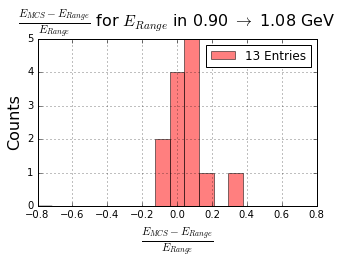
\includegraphics[width=50mm]{Figures/MCS_range_resolution_RecoTracks_slice2.png}}
	\quad
	\subfigure[\textit{Fractional energy difference between 1.45 and 1.63 GeV range energy.}]
	{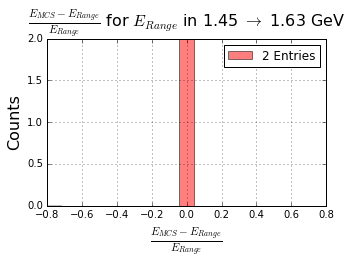
\includegraphics[width=50mm]{Figures/MCS_range_resolution_RecoTracks_slice3.png}}
	}
\caption{\textit{Fractional energy difference for a few representative bins of range energy derived from Figure \ref{MCS_range_energy_RecoTrack_fig}.}}
\label{MCS_range_bias_resolution_RecoTrack_slices_fig}
\end{figure}


\begin{figure}
\centering
\mbox{
	\subfigure[\textit{MCS energy bias as a function of range energy.}]
	{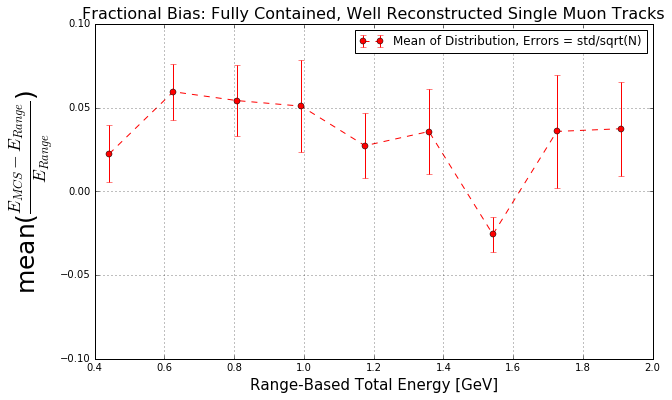
\includegraphics[width=75mm]{Figures/MCS_range_bias_RecoTracks.png}}
	\quad
	\subfigure[\textit{MCS energy resolution as a function of range energy.}]
	{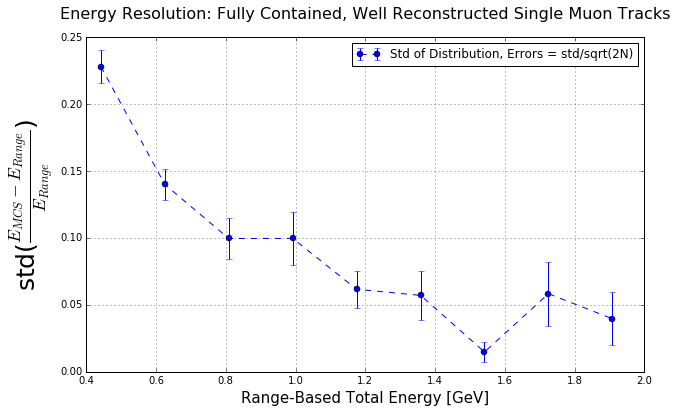
\includegraphics[width=75mm]{Figures/MCS_range_resolution_RecoTracks.png}}
	}
\caption{\textit{MCS energy bias and resolution as a function of range energy for the single muon reconstructed track sample described in Section \ref{RecoTrack_Selection_section}.}}
\label{MCS_range_bias_resolution_RecoTrack_fig}
\end{figure}



\subsubsection{Highland Validation}\label{Highland_Validation_RecoTrack_section}
For this single muon reconstucted track sample, the same Highland validation plot is created in exactly the same way as described in Section \ref{Highland_Validation_MCTrack_section}. For each consecutive pairs of segments, the angular scatter in milliradians divided by the Highland expected RMS in millradians is an entry in the histogram shown in Figure \ref{Highland_validation_RecoTracks_fig}. From this figure we can see that the Highland formula is valid for reconstructed tracks, though the width is slightly smaller than unity. While the gaussian fit does not agree with the underlying histograms as it did in Section \ref{Highland_Validation_MCTrack_section} for {\sc MCTracks}, it is difficult to draw any conclusions about this plot due to extremely limited statistics. Instead the reader is referred to Section \ref{Highland_Validation_MCNuRecoTrack_section} which shows this plot for a higher statistic sample of simulated neutrino-induced muons which are contained.

\begin{figure}[h!]
\begin{center}
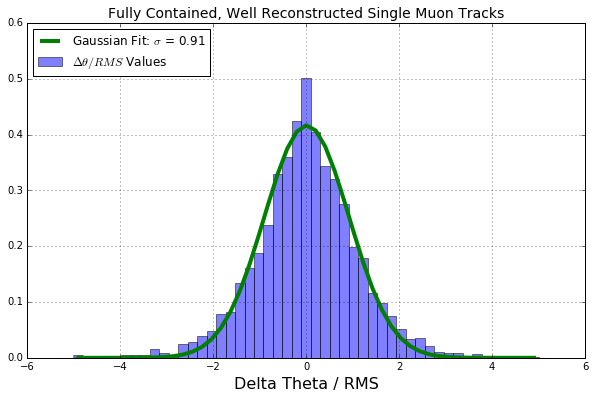
\includegraphics[width=100mm]{Figures/Highland_validation_RecoTracks.png}
\end{center}
\caption{\textit{20cm segment angular deviations divided by expected Highland RMS for the single muon reconstructed track sample described in Section \ref{RecoTrack_Selection_section}.}}
\label{Highland_validation_RecoTracks_fig}
\end{figure}


















% \subsection{Track Reconstruction and Event Selection}
% \subsubsection{Reconstructed Track Description}\label{RecoTrack_section}
% \begin{enumerate}
% \item brief description of pandoraNuPMA algorithm, reference to pandora neutrino2016 documentation
% \item We select events with 1 reconstructed track longer than 1 meter that starts and ends in the correct place (including reversed direction, which we take into account)... correct place means within 5cm of true start and end.
% \item plot of scattering angle / RMS (RMS from range energy)
% \item plot of MCS energy vs true energy
% \item energy resolution in terms of true energy
% \item energy resolution in terms of range energy
% \end{enumerate}

% \subsection{Optimizing Segment Length}
% \begin{enumerate}
% \item using the reconstructed tracks in previous section, overlay energy resolution vs true energy for different segment lengths to pick the best one
% \item also show angle/RMS plot for different segment lengths to show that it only becomes gaussian for longer segment lengths, and that is motivation to pick longer segment lengths.
% \end{enumerate}

% \subsection{Exiting Tracks}
% \begin{enumerate}
% \item reminder that the primary purpose of MCS is to get the energy of exiting tracks
% \item in this section we will use MCTracks that start in fiducial volume and end somewhere outside of it
% \item plot of MCS energy vs true energy
% \item plot: energy resolution in terms of true energy
% \item plot: energy resolution in terms of length of track contained
% \item plot: 2D energy resolution in terms of true energy and length of track contained? dunno if enough stats for that
% \end{enumerate}

% \subsection{MCS as a Tool to Determine Track Direction}
% \begin{enumerate}
% \item here we talk about running MCS on single muon contined reco tracks backwards and forwards and show the likelihood is better for forwards.
% \item i think bruce worked on this first... cite his DocDB about it?
% \end{enumerate}

% \subsection{MCS as a Tool to Determine Reconstruction Quality}
% \begin{enumerate}
% \item here we talk about how broken tracks are a problem, and we show the MCS vs range energy for reco tracks that are broken, and for ones that are not broken, and show that if MCS energy doesn't match range energy one can say that the track is poorly reconstructed.
% \end{enumerate}

% \subsection{MCS as a Tool for Pion/Muon Separation}
% \begin{enumerate}
% \item this is a potential section where we run on pions and muons and somehow claim that MCS can work to separate the two to some extent
% \end{enumerate}



\clearpage

\section{MCS Performance on Truth-Selected Muons from numuCC Events in Simulation}\label{MCBNB_performance_section}


% Executive summary
In this section, studies from this truth-selected simulated BNB numuCC muon sample with {\sc MCTracks} are described. Additionally, similar studies on this sample using automatically reconstructed tracks is described. This section also includes a study justifying that range-based energy is an accurate predictor of true energy for contained muons (with bias less than 1\% and resolution better than 4\%), and therefore can be used in place of true energy so as to compare MC directly to data. The MCS performance on this sample of {\sc MCTracks} is shown to be comparable to that on automatically reconstructed PandoraNuPMA tracks when the track is well reconstructed, with a bias below 5\% and a resolution that varies between 2 and 10\%, performing better for higher momentum (longer) tracks. The resolution is slightly worse for reconstructed tracks than for {\sc MCtracks}. Additionally, the scattering angle of track segments for a given momentum is shown to be similarly gaussian both for {\sc MCTracks} and well reconstructed tracks, in line with the Highland formula prediction.

\subsection{Input Sample}\label{MCBNB_input_sample_section}
The input sample to this portion of the analysis is is 772,000 MCC7 simulated BNB neutrino interactions without any cosmics simulated. These simulated events are run through a fully automated reconstruction chain and then truth information is used to select muons from numuCC interactions which are eligible for MCS analysis. The SAM definition used for this sample is ``prodgenie\_bnb\_nu\_uboone\_mcc7\_reco2''.


\subsection{Fiducial Volume Definition}\label{fidvol_section}
The {\ub} TPC has active volume dimensions of 2.6 m width $\times$ 2.3 m height $\times$ 10.4 m length. For this analysis, a smaller ``fiducial volume'' is defined and referenced throughout this note (for example, in many cases reconstructed tracks are required to be fully contained within the fiducial volume). For reference, the fiducial volume definition used throughout this note is the full TPC volume reduced in by 20 cm from both the cathode plane and the anode wire planes, shifted in 26.5 cm in from both the top and bottom walls of the TPC, shifted in 20 cm from the beam-upstream wall of the TPC, and shifted in 36.8 cm from the downstream wall of the TPC. The reason for this choice of fiducial volume is that it reduces contamination from ``edge effects'' that occur near the walls of the TPC, like electric field distortions and space-charge effects. While the TPC has a total active volume of 62.6 $m^3$, the fiducial volume used in this analysis has a volume of 38.7 $m^3$ or roughly 62\% of the total TPC active volume.









\subsection{Performance with {\sc MCTracks}}\label{MCBNBMCTrack_performance_section}


\subsubsection{MCTrack Description}\label{MCTrack_section}
{\sc MCTrack} objects are made from the output of {\sc geant}4, and are created from {\sc geant}4 energy depositions in the detector. {\sc geant}4 outputs 3D energy depositions in the detector, along with truth information about which parent particles deposited this energy. {\sc MCTracks} are 3D objects which are formed by grouping the energy depositions based on parent particles. Whether a particle in {\sc geant}4 is turned into an {\sc MCTrack} or an {\sc MCShower} (not discussed in this note) is based on truth PDG (for example, muons, protons, and pions always form {\sc MCTracks}).\\

Each {\sc MCTrack} is itself a vector of 3D trajectory points, which are ordered to match the direction of the particle that deposited the energy. Trajectory points are only formed for energy depositions inside of the TPC volume. In general, long {\sc MCTrack}s will have steps separated by up to several centimeters. Each step in an {\sc MCTrack} holds the following information used in this analysis: 3D position, and true energy at that point. Only information within the realm of reconstructable quantities is used in this analysis, with the exception of true energy (which is used for example to quantify a reconstructed energy resolution).\\

Since the output of a nominal reconstruction chain (including hit finding, clustering, matching across planes, etc.) are 3D tracks, {\sc MCTracks} can be studied in an analysis in the exact same way as a reconstructed track would be. {\sc MCTracks} can be thought of as perfectly reconstructed tracks, where each trajectory point along the track is a true 3D energy deposition inside of the {\ub} TPC.\\

Since {\sc MCTracks} are formed from true 3D energy depositions and not from wire signals on drift electrons, {\sc MCTracks} are insensitive to broken wires, noise, and other simulated detector effects.\\

It is worth noting that delta rays eminating from muon tracks are relevant for MCS calculations. Here, delta rays form {\sc MCShowers} and are therefore invisible to this analysis. This is the same as assuming the reconstructed tracks have perfectly removed charge from delta rays in their algorithms.




\subsubsection{Event Selection}\label{MCBNBMCTrack_eventselection_section}
The event selection for this subanalysis is truth based. The fiducial volume used in this subanalysis is the same as is used throughout the note, defined in Section \ref{fidvol_section}. Beginning with the 772,000 events in the sample, the cuts placed are:

\begin{itemize}
\item There is one neutrino interaction in the event (770,241 events remain).
\item The neutrino interaction is of type charged-current (559,348 events remain).
\item The neutrino interaction occurs within the fiducial volume (152,214 events remain).
\item The interacting neutrino is type $\nu_\mu$ (149,684 events remain).
\item The {\sc MCTrack} associated with the outgoing muon from the interaction is fully contained within the fiducial volume (50,537 events remain).
\item The {\sc MCTrack} associated with the outgoing muon from the interaction is at least one meter in length (23,378 events remain).
\item The {\sc MCTrack} associated with the outgoing muon from the interaction does not decay in flight (this cut is implemented by requiring the {\sc MCTrack}'s total energy at its final trajectory point is equal to the muon mass) (23,342 events remain).
\end{itemize}
After these additional cuts are placed, 23342 events ({\sc MCTracks}) remain for MCS analysis. The energy and angle distributions for these 23342 muons can be seen in Figure \ref{BNBmuon_energy_angle_fig}. It should be noted that any computed metrics from this sample (and therefore any other BNB sample) have convolved any effects of performance differences as a function of angle.\\

\begin{figure}
\centering
\mbox{
	\subfigure[\textit{Muon energy distribution.}]
	{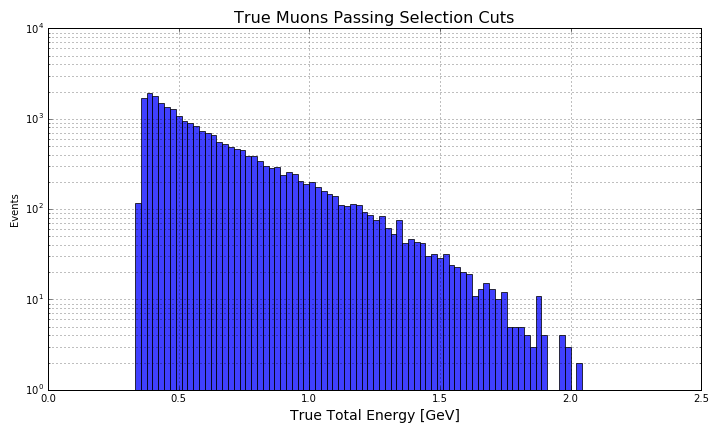
\includegraphics[width=75mm]{Figures/MCBNBMCTrack_EnergySpectrum.png}}
	\quad
	\subfigure[\textit{Muon theta angle (angle with respect to the beam direction) distribution.}]
	{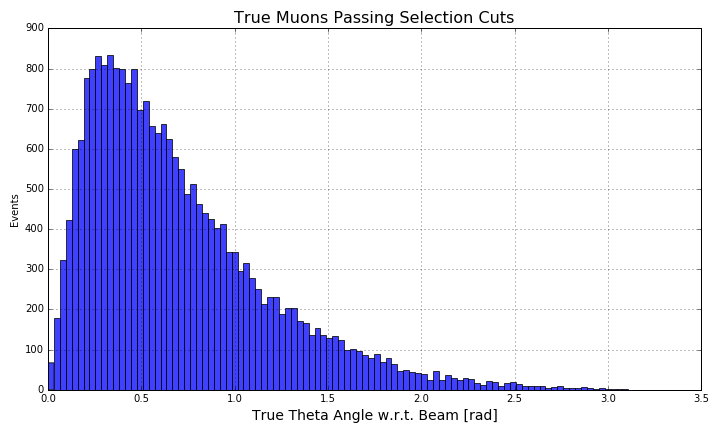
\includegraphics[width=75mm]{Figures/MCBNBMCTrack_AngleSpectrum.png}}
	}
\caption{\textit{Energy and angle distributions for muons from numuCC interactions in {\ub} simulation passing cuts described in Section \ref{MCBNBMCTrack_eventselection_section}.}}
\label{BNBmuon_energy_angle_fig}
\end{figure}



\subsubsection{Range Energy Validation}\label{Range_Energy_Validation_section}
With this sample of {\sc MCTracks}, it is possible to quantify MCS energy (momentum) resolution as a function of true energy (momentum). However, in actual {\ub} data there is obviously no true momentum with which to compare. The additional momentum handle that is used in data for contained tracks is range-based energy. The stopping power of muons in liquid argon is well described by the particle data group\cite{PDG_spline_table}. By using a linear interpolation between points in the cited PDG stopping power table, the start-to-end straight-line length of a track can be used to reconstruct the muon's total energy with good accuracy. Figure \ref{true_range_energy_MCTrack_fig} shows a comparison of range energy to true energy for this sample. \\

In order to compute a bias and a resolution, Figure \ref{true_range_energy_MCTrack_fig} is sliced in bins of true muon energy and a histogram of the fractional energy difference ($\frac{E_{range} - E_{true}}{E_{true}}$) is created for each bin. This distribution is shown for three representative bins in Figure \ref{true_range_bias_resolution_MCTrack_slices_fig}, along with the gaussian fit to each.  The mean ($\mu$) of each gaussian fit is used to compute a bias as a function of true energy, while the width ($\sigma$) of each distribution is used to compute a resolution. Figure \ref{true_range_bias_resolution_MCTrack_fig} shows the bias and resolution for the range-based energy reconstruction method. It can be seen that the bias is negligible and the resolution for this method of energy reconstruction is on the order of 2-4\%. Based on this figure, it is clear that range-based energy (and therefore range-based momentum) is a good handle on the true energy (momentum) of a reconstructed muon track in {\ub} data, assuming that track is well reconstructed in terms of length.

\begin{figure}[ht!]
\begin{center}
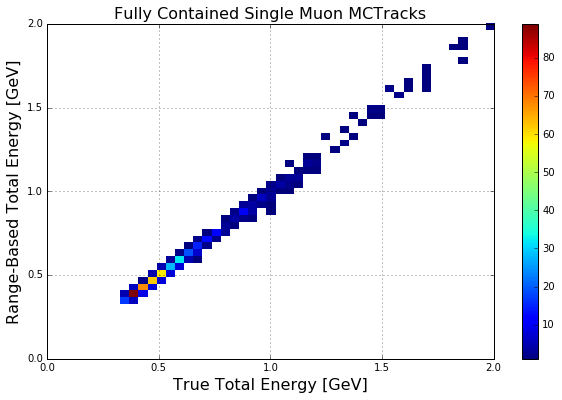
\includegraphics[width=100mm]{Figures/true_range_comparison_MCTracks.png}
\end{center}
\caption{\textit{Range based energy versus true energy for the {\sc MCTrack} sample described in Section \ref{MCBNBMCTrack_eventselection_section}.}}
\label{true_range_energy_MCTrack_fig}
\end{figure}

\begin{figure}
\centering
\mbox{
	\subfigure[\textit{Fractional energy difference between 0.35 and 0.53 GeV true energy.}]
	{\includegraphics[width=50mm]{Figures/{true_range_resolution_MCBNBMCTrack_slice_0.35_0.53}.png}}
	\quad
	\subfigure[\textit{Fractional energy difference between 0.90 and 1.08 GeV true energy.}]
	{\includegraphics[width=50mm]{Figures/{true_range_resolution_MCBNBMCTrack_slice_0.90_1.08}.png}}
	\quad
	\subfigure[\textit{Fractional energy difference between 1.45 and 1.63 GeV true energy.}]
	{\includegraphics[width=50mm]{Figures/{true_range_resolution_MCBNBMCTrack_slice_1.45_1.63}.png}}
	}
\caption{\textit{Fractional energy difference for a few representative bins of true energy derived from Figure \ref{true_range_energy_MCTrack_fig}.}}
\label{true_range_bias_resolution_MCTrack_slices_fig}
\end{figure}




\begin{figure}
\centering
\mbox{
	\subfigure[\textit{Range energy bias as a function of true energy. The vertical error bars are computed as $\frac{\sigma_{fit}}{\sqrt{N}}$, and the horizontal error bars indicate bin width.}]
	{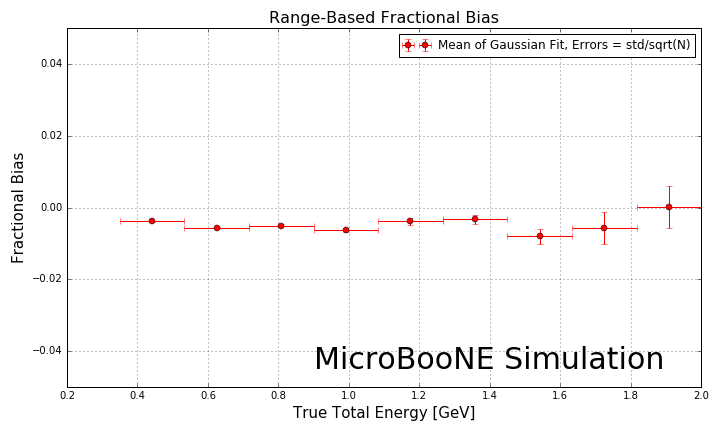
\includegraphics[width=75mm]{Figures/true_range_bias_MCBNBMCTrack.png}}
	\quad
	\subfigure[\textit{Range energy resolution as a function of true energy. The vertical error bars are computed as $\frac{\sigma_{fit}}{\sqrt{2N}}$, and the horizontal error bars indicate bin width.}]
	{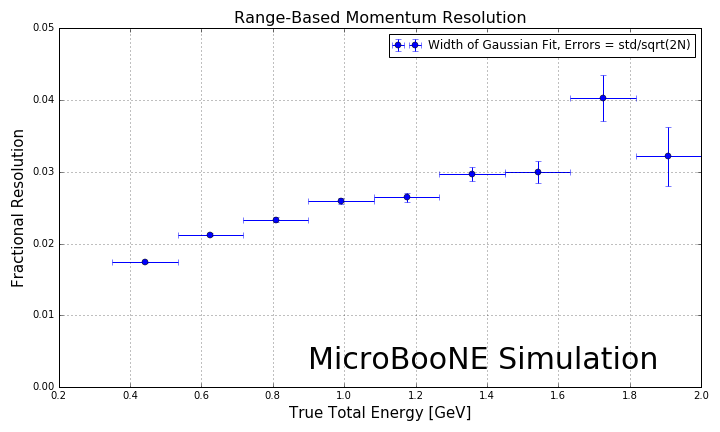
\includegraphics[width=75mm]{Figures/true_range_resolution_MCBNBMCTrack.png}}
	}
\caption{\textit{Range energy and true energy bias and resolution for the {\sc MCTrack} sample described in Section \ref{MCBNBMCTrack_eventselection_section}.}}
\label{true_range_bias_resolution_MCTrack_fig}
\end{figure}







\subsubsection{MCS Momentum Validation}\label{MCS_Momentum_Validation_MCTrack_section}
For this sample of {\sc MCTracks}, only the 3D trajectory points of each {\sc MCTrack} are used as input to the MCS code, described in Section \ref{MCS_technique_section}. The resulting MCS momentum versus range-based momentum can be seen in Figure \ref{MCS_range_momentum_MCTrack_fig}. Range momentum is used here instead of true momentum in order to make this plot more directly comparable with the same analysis on data where true momentum is not accessible. In order to compute a bias and a resolution, Figure \ref{MCS_range_momentum_MCTrack_fig} is sliced in bins of range momentum and a histogram of the fractional momentum difference ($\frac{p_{MCS}^{-1} - p_{range}^{-1}}{p_{range}^{-1}}$) is created for each bin\footnote{The choice of using inverse momentum is justified in Appendix \ref{inverse_p_justification_section}.}. This distribution is shown for three representative bins in Figure \ref{MCS_range_bias_resolution_MCTrack_slices_fig}, along with the gaussian fit to each.  The mean ($\mu$) of each gaussian fit is used to compute a bias as a function of range momentum, while the width ($\sigma$) of each distribution is used to compute a resolution. The bias and resolution for this momentum reconstruction method shown in Figure \ref{MCS_range_bias_resolution_MCTrack_fig}. This figure indicates a bias in the MCS momentum resolution on the order of a few percent, with a resolution that decreases from about 9\% for contained {\sc MCTracks} with true total momentum around 0.5 GeV (which corresponds to a length of about 1.7 meters) to below 3\% for contained {\sc MCTracks} with true total momentum greater than 0.8 GeV (which corresponds to a length of about 3.1 meters).


\begin{figure}[ht!]
\begin{center}
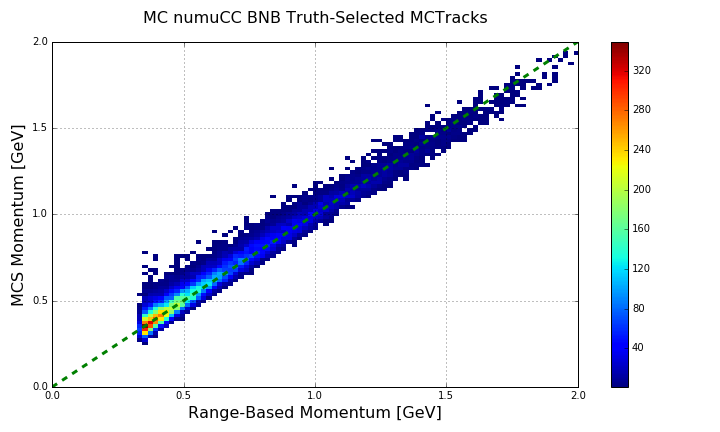
\includegraphics[width=100mm]{Figures/MCS_range_comparison_MCBNBMCTrack.png}
\end{center}
\caption{\textit{MCS computed momentum versus range momentum for the {\sc MCTrack} sample described in Section \ref{MCBNBMCTrack_eventselection_section}. Note the cutoff at around 0.3 GeV range-based momentum is caused by the minimum track length of 100 centimenter requirement.}}
\label{MCS_range_momentum_MCTrack_fig}
\end{figure}

\begin{figure}
\centering
\mbox{
	\subfigure[\textit{Fractional momentum difference between 0.35 and 0.53 GeV range momentum.}]
	{\includegraphics[width=50mm]{Figures/{MCS_range_resolution_MCBNBMCTrack_slice_0.35_0.53}.png}}
	\quad
	\subfigure[\textit{Fractional momentum difference between 0.90 and 1.08 GeV true momentum.}]
	{\includegraphics[width=50mm]{Figures/{MCS_range_resolution_MCBNBMCTrack_slice_0.90_1.08}.png}}
	\quad
	\subfigure[\textit{Fractional momentum difference between 1.45 and 1.63 GeV true momentum.}]
	{\includegraphics[width=50mm]{Figures/{MCS_range_resolution_MCBNBMCTrack_slice_1.45_1.63}.png}}
	}
\caption{\textit{Fractional momentum difference for a few representative bins of range momentum derived from Figure \ref{MCS_range_momentum_MCTrack_fig}.}}
\label{MCS_range_bias_resolution_MCTrack_slices_fig}
\end{figure}


\begin{figure}
\centering
\mbox{
	\subfigure[\textit{MCS momentum bias as a function of range momentum. The vertical error bars are computed as $\frac{\sigma_{fit}}{\sqrt{N}}$, and the horizontal error bars indicate bin width.}]
	{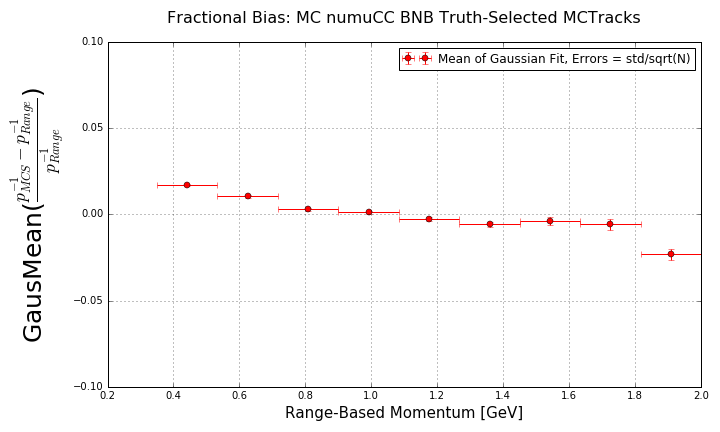
\includegraphics[width=75mm]{Figures/MCS_range_bias_MCBNBMCTrack.png}}
	\quad
	\subfigure[\textit{MCS momentum resolution as a function of range momentum. The vertical error bars are computed as $\frac{\sigma_{fit}}{\sqrt{2N}}$, and the horizontal error bars indicate bin width.}]
	{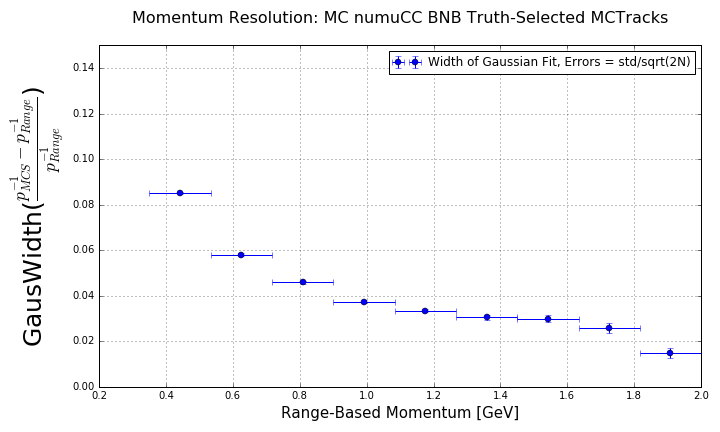
\includegraphics[width=75mm]{Figures/MCS_range_resolution_MCBNBMCTrack.png}}
	}
\caption{\textit{MCS momentum bias and resolution as a function of range momentum for the {\sc MCTrack} sample described in Section \ref{MCBNBMCTrack_eventselection_section}.}}
\label{MCS_range_bias_resolution_MCTrack_fig}
\end{figure}



\subsubsection{Highland Validation}\label{Highland_Validation_MCTrack_section}
For a given track segment momentum and length, 98\% of the angular scatter deviations should be gaussian with an RMS described by the Highland equation (Equation \ref{highland_eqtn}), while the remaining 2\% are larger angle Rutherford scatters\cite{highland}\footnote{This is not actually taken into account explicitly in the current algorithm implementation}. Therefore, a histogram of track segment angular deviations divided by the RMS predicted by the Highland equation should be gaussian with a width of unity. In this section, we validate this claim.\\

For each 10 cm segment of each {\sc MCTrack} in this single muon sample, the momentum of the muon at the start of that segment is estimated by taking the computed MCS momentum and subtracting out momentum lost in the track upstream of the start of this segment, assuming the track was minimally ionizing as described in Equation \ref{segment_E_equation}. The segment momentum, along with the segment length, is converted into an expected RMS angular deviation by way of Equation \ref{highland_eqtn}. For each consecutive pair of segments, the angular scatter in milliradians divided by the Highland expected RMS in millradians is an entry in the histogram shown in Figure \ref{Highland_validation_MCTracks_fig}. From this figure we can see that the Highland formula is valid for {\sc MCTracks}, as the gaussian fit agrees well with the underlying histogram.

\begin{figure}[ht!]
\begin{center}
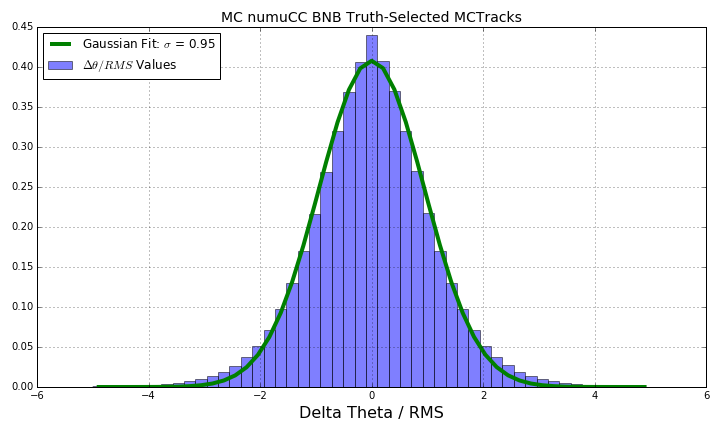
\includegraphics[width=100mm]{Figures/Highland_validation_MCBNBMCTrack.png}
\end{center}
\caption{\textit{10 cm segment angular deviations divided by expected Highland RMS for the single muon {\sc MCTrack} sample described in Section \ref{MCBNBMCTrack_eventselection_section}.}}
\label{Highland_validation_MCTracks_fig}
\end{figure}




























\subsection{Performance with Reconstructed Tracks}\label{MCBNBRecoTrack_performance_section}

\subsubsection{Event Selection}\label{MCBNBRecoTrack_eventselection_section}
The event selection for this subanalysis is identical to that described in Section \ref{MCBNBMCTrack_eventselection_section} with one additional cut. The additional cut is requiring that there is a reconstructed track which starts within 3 cm of the start and ends within 3 cm of the end of the aforementioned {\sc MCTrack} (or vice-versa). This cut is requiring that the track is well reconstructed in terms of position (direction is taken into account later). 13810 events pass this cut, down from the 23342 previously.

\subsubsection{MCS Momentum Validation}\label{MCS_Momentum_Validation_MCBNBRecoTrack_section}
For this sample of reconstructed tracks, only the 3D trajectory points of each reconstructed track are used as input to the MCS code, described in Section \ref{MCS_technique_section}. The resulting MCS momentum versus range-based momentum for this sample of reconstructed tracks without any cuts other than those described in Section \ref{MCBNBRecoTrack_eventselection_section} can be seen in Figure \ref{MCS_range_momentum_MCBNBRecoTrack_fig}. \\

In order to compute a bias and a resolution, Figure \ref{MCS_range_momentum_MCBNBRecoTrack_fig} is sliced in bins of range momentum and a histogram of the fractional momentum difference ($\frac{p_{MCS}^{-1} - p_{range}^{-1}}{p_{range}^{-1}}$) is created for each bin\footnote{The choice of using inverse momentum is justified in Appendix \ref{inverse_p_justification_section}}. This distribution is shown for three representative bins in Figure \ref{MCS_range_bias_resolution_MCBNBRecoTrack_slices_fig}, along with the gaussian fit to each.  The mean ($\mu$) of each gaussian fit is used to compute a bias as a function of range momentum, while the width ($\sigma$) of each distribution is used to compute a resolution. The bias and resolution for this momentum reconstruction method shown in Figure \ref{MCS_range_bias_resolution_MCBNBRecoTrack_fig}. This figure indicates a bias in the MCS momentum resolution on the order of a few percent, with a resolution that decreases from about 9\% for contained tracks with true total momentum around 0.5 GeV (which corresponds to a length of about 1.7 meters) to below 7\% for contained tracks with true total momentum greater than 0.8 GeV (which corresponds to a length of about 3.1 meters). This agrees reasonably well with the analogous plots created from simulated single muons with {\sc MCTracks} (Figure \ref{MCS_range_bias_resolution_MCTrack_fig}).


\begin{figure}[ht!]
\begin{center}
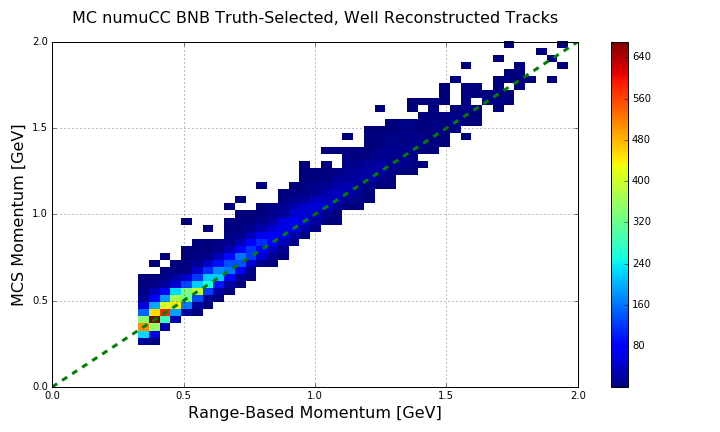
\includegraphics[width=100mm]{Figures/MCS_range_comparison_MCBNBRecoTrack.png}
\end{center}
\caption{\textit{MCS computed momentum versus range momentum for the truth-selected simulated fully contained, well reconstructed muon tracks from numu charged current events.}}
\label{MCS_range_momentum_MCBNBRecoTrack_fig}
\end{figure}


\begin{figure}
\centering
\mbox{
	\subfigure[\textit{Fractional momentum difference between 0.35 and 0.53 GeV range momentum.}]
	{\includegraphics[width=50mm]{Figures/{MCS_range_resolution_MCBNBRecoTrack_slice_0.35_0.53}.png}}
	\quad
	\subfigure[\textit{Fractional momentum difference between 0.90 and 1.08 GeV range momentum.}]
	{\includegraphics[width=50mm]{Figures/{MCS_range_resolution_MCBNBRecoTrack_slice_0.90_1.08}.png}}
	\quad
	\subfigure[\textit{Fractional momentum difference between 1.45 and 1.63 GeV range momentum.}]
	{\includegraphics[width=50mm]{Figures/{MCS_range_resolution_MCBNBRecoTrack_slice_1.45_1.63}.png}}
	}

\caption{\textit{Fractional momentum difference for a few representative bins of range momentum derived from Figure \ref{MCS_range_momentum_MCBNBRecoTrack_fig}.}}
\label{MCS_range_bias_resolution_MCBNBRecoTrack_slices_fig}
\end{figure}


\begin{figure}
\centering
\mbox{
	\subfigure[\textit{MCS momentum bias as a function of range momentum. The vertical error bars are computed as $\frac{\sigma_{fit}}{\sqrt{N}}$, and the horizontal error bars indicate bin width.}]
	{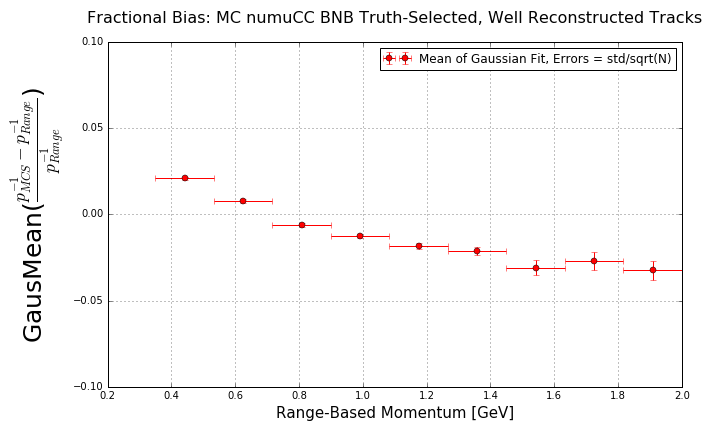
\includegraphics[width=75mm]{Figures/MCS_range_bias_MCBNBRecoTrack.png}}
	\quad
	\subfigure[\textit{MCS momentum resolution as a function of range momentum. The vertical error bars are computed as $\frac{\sigma_{fit}}{\sqrt{2N}}$, and the horizontal error bars indicate bin width.}]
	{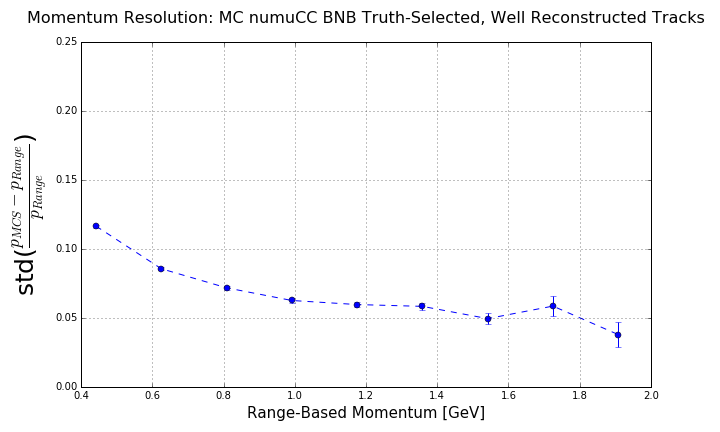
\includegraphics[width=75mm]{Figures/MCS_range_resolution_MCBNBRecoTrack.png}}
	}
\caption{\textit{MCS momentum bias and resolution as a function of range momentum for the truth-selected simulated fully contained, well reconstructed muon tracks from numu charged current events.}}
\label{MCS_range_bias_resolution_MCBNBRecoTrack_fig}
\end{figure}



\subsubsection{Highland Validation}\label{Highland_Validation_MCBNBRecoTrack_section}
For this sample of tracks, the same Highland validation plot is created in exactly the same way as described in Section \ref{Highland_Validation_MCTrack_section}. For each consecutive pair of segments, the angular scatter in milliradians divided by the Highland expected RMS in millradians is an entry in the histogram shown in Figure \ref{Highland_validation_MCBNBRecoTrack_fig}. From this figure we can see that the Highland formula is valid for well reconstructed tracks in simulation when 10 cm segments are used.

\begin{figure}[ht!]
\begin{center}
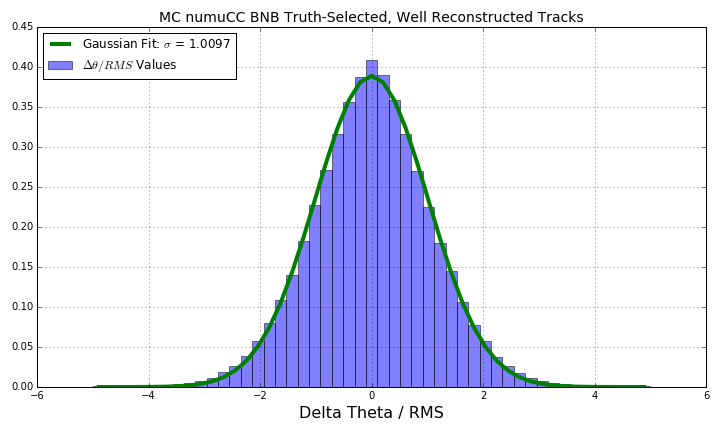
\includegraphics[width=100mm]{Figures/Highland_validation_MCBNBRecoTrack.png}
\end{center}
\caption{\textit{10 cm segment angular deviations divided by expected Highland RMS for the sample of well reconstructed, neutrino induced muons in simulation.}}
\label{Highland_validation_MCBNBRecoTrack_fig}
\end{figure}




\clearpage
%%%% SIGNAL SECTION %%%%
\section{MCS Performance on Automatically Selected Muons from numuCC Events With Cosmics in Simulation}\label{MC_performance_section}

\subsection{Input sample}\label{MC_BNB_input_sample_section}
The input sample to this portion of the analysis is roughly 190,000 MCC7 simulated BNB neutrino interactions with CORSIKA cosmics as used by the CCInclusive group and descibed in their interal note\cite{CCIncInternalNote}. These simulated events are run through a fully automated reconstruction chain and then a fully automated event selection routine described in Section \ref{MC_BNB_eventselection_section}. The SAM definition used for this sample is ``prodgenie\_bnb\_nu\_cosmic\_uboone\_mcc7\_reco2''.

\subsection{Event selection}\label{MC_BNB_eventselection_section}
The event selection algorithms used are designed to locate $\nu_\mu$ charged-current interactions, where at least one muon track exits the interaction vertex. The event selection is described in detail in Section 6.2.1 of the {\ub} CCInclusive internal note (``Selection IIA: track multiplicity 2 (or larger) and no containment requirement'')\cite{CCIncInternalNote}  but the main points will be recapped here. The selection takes as input reconstructed vertices created by the ``pmtrack'' producer module, reconstructed tracks created by the ``pandoraNuPMA'' track producer module, and optical hits produced by the ``opFlashSat'' producer module. The following selection cuts are placed to isolate $\nu_\mu$ charged-current interactions:
\begin{enumerate}
\item The event must have at least one flash inside of the BNB beam-spill window brighter than 50 PE.
\item Two or more reconstructed tracks must originate from the same reconstructed vertex within the fiducial volume (defined in Section \ref{fidvol_section}).
\item The tracks must overlap within a 70 cm buffer in the drift (z) direction of the center of the reconstructed optical flash.
\item For events with exactly two tracks originating from the vertex, additional calorimetric-based cuts are applied to mitigate backgrounds from in-time cosmics which produce Michel electrons that get reconstructed as a track.
\end{enumerate}

After these event selection cuts are placed, further cuts are placed to isolate single tracks that are eligible for this MCS analysis. 
\begin{enumerate}
\item The longest track is assumed to be the muon, and it is the only track studied in this analysis. 
\item This track must be at least one meter in length, and it also must match with an {\sc MCTrack} (Section \ref{MCTrack_section}) originating from the true neutrino interaction in the event. Here, ``match'' means that the start of the reconstructed track is within 3 cm of the start of the {\sc MCTrack}, and the end of the reconstructed track is within 3 cm of the end of the {\sc MCTrack} (or vice-versa).
\item The longest track must be fully contained within the fiducial volume.
\end{enumerate}

After these additional cuts are placed, 1613 events (tracks) remain for MCS analysis. It should be known that there are some inherent pion and proton mis-identification (MID) backgrounds in this sample after these cuts are placed. 88\% of the time the identified track is truly a muon. Protons and pions make up the remaining MIDs with 8.6\% and 3.4\% respectively.


% Let's be honest with ourselves this pie chart is unnecessary and should just be described in one sentence.
% \begin{figure}[ht!]
% \begin{center}
% \includegraphics[width=100mm]{Figures/MCBNBSelectedRecoTrack_MID_piechart.png}
% \end{center}
% \caption{\textit{A pie chart summarizing the types and rates of different MIDs inherent in this sample. 88\% of the time the identified track is truly a muon. Protons and pions make up the remaining MID rates with 8.6\% and 3.4\% respectively.}}
% \label{MCBNBSelectedRecoTrack_MID_piechart_fig}
% \end{figure}


\subsection{MCS Momentum Validation}\label{MCS_Momentum_Validation_MCBNBSelectedRecoTrack_section}
For this sample of reconstructed tracks, only the 3D trajectory points of each reconstructed track are used as input to the MCS code, described in Section \ref{MCS_technique_section}. The resulting MCS momentum versus range-based momentum without any cuts other than those described in Section \ref{MC_BNB_eventselection_section} can be seen in Figure \ref{MCS_range_momentum_MCBNBSelectedRecoTrack_noPDGcut_fig}. The off-diagonal visible in this figure (where MCS momentum greatly overestimates range momentum) is caused primarily by MIDs, most commonly where the longest track is a proton. Note that there are no ``broken tracks'' (which is another not-yet-discussed possible explanation for the off-diagonal) because of the track-{\sc MCTrack} matching requirement described in Section \ref{MC_BNB_eventselection_section}. Figure \ref{MCS_range_momentum_MCBNBSelectedRecoTrack_withPDGcuts_fig} divides Figure \ref{MCS_range_momentum_MCBNBSelectedRecoTrack_noPDGcut_fig} into those events in which the MCTrack matched to the reconstructed track is a proton, a pion, or a muon. From this figure it is clear comparing MCS momentum to range momentum for contained tracks will provide a handle on separating muon tracks from proton tracks in data (though it is hard to make similar conclusions about pions due to limited statistics in this study).\\

In order to compute a bias and a resolution, Figure \ref{MCS_range_momentum_MCBNBSelectedRecoTrack_muononly_fig} is sliced in bins of range momentum and a histogram of the fractional momentum difference ($\frac{p_{MCS}^{-1} - p_{range}^{-1}}{p_{range}^{-1}}$) is created for each bin. Note that the inverse of the momentum is used rather than the momentum because this distribution is more gaussian distributed. Also note that this fractional momentum difference using inverse of momentum is algebraically equivalent to ($\frac{p_{range} - p_{MCS}}{p_{MCS}}$). This distribution is shown for three representative bins in Figure \ref{MCS_range_bias_resolution_MCBNBSelectedRecoTrack_slices_fig}, along with the gaussian fit to each.  The mean ($\mu$) of each gaussian fit is used to compute a bias as a function of range momentum, while the width ($\sigma$) of each distribution is used to compute a resolution. The bias and resolution for this momentum reconstruction method is shown in Figure \ref{MCS_range_bias_resolution_MCBNBSelectedRecoTrack_fig}. This figure indicates a bias in the MCS momentum resolution on the order of a few percent, with a resolution that decreases from about 10\% for contained tracks with true total momentum around 0.5 GeV (which corresponds to a length of about 1.7 meters) to below 7\% for contained tracks with true total momentum greater than 0.8 GeV (which corresponds to a length of about 3.1 meters). This agrees well with the analogous plots created from simulated single muons with {\sc MCTracks} (Figure \ref{MCS_range_bias_resolution_MCTrack_fig}).


\begin{figure}[ht!]
\begin{center}
\includegraphics[width=100mm]{Figures/MCS_range_comparison_MCBNBSelectedRecoTrack.png}
\end{center}
\caption{\textit{MCS computed momentum versus range momentum for the automatically selected simulated neutrino-induced fully contained, well reconstructed muon sample without any additional cuts to mitigate MIDs.}}
\label{MCS_range_momentum_MCBNBSelectedRecoTrack_noPDGcut_fig}
\end{figure}

\begin{figure}
\centering
\mbox{
	\subfigure[\textit{The subset of events in Figure \ref{MCS_range_momentum_MCBNBSelectedRecoTrack_noPDGcut_fig} in which the true identity of the track is a proton.}]
	{\includegraphics[width=50mm]{Figures/MCS_range_momentum_MCBNBSelectedRecoTrack_2212.png}}
	\quad
	\subfigure[\textit{The subset of events in Figure \ref{MCS_range_momentum_MCBNBSelectedRecoTrack_noPDGcut_fig} in which the true identity of the track is a pion.}]
	{\includegraphics[width=50mm]{Figures/MCS_range_momentum_MCBNBSelectedRecoTrack_211.png}}
	\quad
	\subfigure[\textit{The subset of events in Figure \ref{MCS_range_momentum_MCBNBSelectedRecoTrack_noPDGcut_fig} in which the true identity of the track is a muon.}\label{MCS_range_momentum_MCBNBSelectedRecoTrack_muononly_fig}]
	{\includegraphics[width=50mm]{Figures/MCS_range_momentum_MCBNBSelectedRecoTrack_13.png}}
	}
\caption{\textit{MCS computed momentum versus range momentum for the selected neutrino-induced, well reconstructed fully contained muon sample in simulation broken up by true particle identity of the track.}}
\label{MCS_range_momentum_MCBNBSelectedRecoTrack_withPDGcuts_fig}
\end{figure}


\begin{figure}
\centering
\mbox{
	\subfigure[\textit{Fractional momentum difference between 0.35 and 0.53 GeV range momentum.}]
	{\includegraphics[width=50mm]{Figures/{MCS_range_resolution_MCBNBSelectedRecoTrack_slice_0.35_0.53}.png}}
	\quad
	\subfigure[\textit{Fractional momentum difference between 0.90 and 1.08 GeV range momentum.}]
	{\includegraphics[width=50mm]{Figures/{MCS_range_resolution_MCBNBSelectedRecoTrack_slice_0.90_1.08}.png}}
	\quad
	\subfigure[\textit{Fractional momentum difference between 1.45 and 1.63 GeV range momentum.}]
	{\includegraphics[width=50mm]{Figures/{MCS_range_resolution_MCBNBSelectedRecoTrack_slice_1.45_1.63}.png}}
	}

\caption{\textit{Fractional momentum difference for a few representative bins of range momentum derived from Figure \ref{MCS_range_momentum_MCBNBSelectedRecoTrack_muononly_fig}.}}
\label{MCS_range_bias_resolution_MCBNBSelectedRecoTrack_slices_fig}
\end{figure}


\begin{figure}
\centering
\mbox{
	\subfigure[\textit{MCS momentum bias as a function of range momentum.}]
	{\includegraphics[width=75mm]{Figures/MCS_range_bias_MCBNBSelectedRecoTrack.png}}
	\quad
	\subfigure[\textit{MCS momentum resolution as a function of range momentum.}]
	{\includegraphics[width=75mm]{Figures/MCS_range_resolution_MCBNBSelectedRecoTrack.png}}
	}
\caption{\textit{MCS momentum bias and resolution as a function of range momentum for the selected, well reconstructed neutrino-induced muons in {\ub} simulation.}}
\label{MCS_range_bias_resolution_MCBNBSelectedRecoTrack_fig}
\end{figure}



\subsection{Highland Validation}\label{Highland_Validation_MCBNBSelectedRecoTrack_section}
For this sample of contained, automatically selected, well-reconstructed neutrino-induced tracks, the same Highland validation plot is created in exactly the same way as described in Section \ref{Highland_Validation_MCTrack_section}. For each consecutive pair of segments, the angular scatter in milliradians divided by the Highland expected RMS in millradians is an entry in the histogram shown in Figure \ref{Highland_validation_MCBNBSelectedRecoTracks_fig}. From this figure we can see that the Highland formula is valid for automatically selected, well reconstructed neutrino-induced muon tracks in simulation.

\begin{figure}[ht!]
\begin{center}
\includegraphics[width=100mm]{Figures/Highland_validation_MCBNBSelectedRecoTrack.png}
\end{center}
\caption{\textit{10 cm segment angular deviations divided by expected Highland RMS for the sample of well reconstructed, neutrino induced muons in simulation.}}
\label{Highland_validation_MCBNBSelectedRecoTracks_fig}
\end{figure}
\clearpage
%%%% SIGNAL SECTION %%%%
\section{MCS Performance on Automatically Selected Muons from numuCC Events in MicroBooNE Data}\label{data_performance_section}

\subsection{Input Sample}
The input sample to this portion of the analysis is roughly 5e19 POT worth of triggered BNB neutrino interactions in {\ub} data as used by the CCInclusive group and descibed in their interal note\cite{CCIncInternalNote}. These events are run through the same fully automated reconstruction chain and event selection routine described in Section \ref{MC_BNB_input_sample_section}. The SAM definition used for this sample is ``prod\_bnb\_reco\_neutrino2016\_beamfilter\_goodruns\_v5''.

\subsection{Event Selection}
The exact same event selection cuts are used to identify $\nu_\mu$ charged-current events in this data sample as described in Section \ref{MC_BNB_eventselection_section}. The fiducial volume used in this subanalysis is the same as is used throughout the note, defined in Section \ref{fidvol_section}. The same further cuts to isolate the subset of those events viable for MCS analysis are also placed, with the exception of the cut requiring the reconstructed track matches well with an {\sc MCTrack} in the event (as there are no {\sc MCTracks} in real data). In order to accommodate for this difference, a hand scan of the selected events was conducted.\\

After the event selection cuts, the minimum track length cut, and the containment cuts were placed, 598 events (tracks) remained. Each of these events (tracks) were scanned by hand with an interactive event display. What was shown to the scanner (David Kaleko) were three two-dimensional displays with the raw-wire signals on them. Overlaid on each display was the 2D projection of the 3D reconstructed track and vertex. The scanner looked to ensure the track was well reconstructed (it started within a few cm of the vertex and ended within a few cm of the end of the wire-signal track or vice-versa in all three planes). Additionally the scanner looked for obvious MID topologies like cosmic rays inducing Michel electrons at the reconstructed neutrino vertex (for example when a clear Bragg peak is visible at the neutrino vertex) and also for obvious MID topologies where the track is likely a pion (for example if it charge-exchanges and creates a clear neutral pion decay topology). In general, the scanner chose to be conservative in the sense that if the track didn't look very clearly like a muon from a $\nu_\mu$ charged-current event, the track (event) was removed from the analysis. The purpose of searching for MIDs is to attempt to reproduce the truth-based removal of cosmic, pion, and proton MIDs that is ultimately done in Section \ref{MC_performance_section} so as to make an apples-to-apples data/MC comparison.\\

A sample event that was removed by the hand scanner is shown in Figure \ref{bad_evd_fig_1}. Only one two-dimensional display is shown (from the collection plane wires), while the 2D projection of the 3D track is shown in black. The 2D projection of the 3D reconstructed neutrino vertex is shown as a small cyan dot near the bottom left of the image. It is clear that the reconstructed track starts in the correct place, but it is truncated and stops before the end of the track. This track was deemed ``poorly reconstructed'' and was therefore removed from the analysis. A second sample event that was removed by the hand scanner is shown in Figure \ref{bad_evd_fig_2}. This event was deemed some form of unknown MID. The reconstructed track matches wire signals well, but this event does not appear to be a clean $\nu_\mu$ charged-current event, with at least one neutral pion decay visible near the center of the track. A sample event that was deemed acceptable is shown in Figure \ref{good_evd_fig_1}.

\begin{figure}[ht!]
\begin{center}
\includegraphics[width=100mm]{Figures/static_figs/bad_evd_1.png}
\end{center}
\caption{\textit{A hand-scanned data event that was deemed ``poorly reconstructed'' and removed from this analysis. The 2D projection of the 3D reconstructed track (shown in black overlaid on raw wire signals) clearly stops before it reaches the end of the particle's trajectory.}}
\label{bad_evd_fig_1}
\end{figure}

\begin{figure}[ht!]
\begin{center}
\includegraphics[width=100mm]{Figures/static_figs/bad_evd_2.png}
\end{center}
\caption{\textit{A hand-scanned data event that was deemed some form of MID and removed from this analysis. The 2D projection of the 3D reconstructed track (shown in black overlaid on raw wire signals) matches raw wire signals well, but this event does not appear to be a clean $\nu_\mu$ charged-current event, with at least one neutral pion decay visible near the center of the track.}}
\label{bad_evd_fig_2}
\end{figure}

\begin{figure}[ht!]
\begin{center}
\includegraphics[width=100mm]{Figures/static_figs/good_evd_1.png}
\end{center}
\caption{\textit{A hand-scanned data event that was deemed acceptable for MCS analysis. The track looks well reconstructed, and the wire signals indicate that the particle is likely a muon, and a clear Bragg peak can be seen at the end of the track indicating the track is well contained.}}
\label{good_evd_fig_1}
\end{figure}

\subsection{MCS Momentum Validation}\label{MCS_Momentum_Validation_DataRecoTrack_section}
The MCS momentum versus range-based momentum \textit{without any additional hand-scan reconstruction quality checks} can be seen in Figure \ref{MCS_range_momentum_DataRecoTrack_nohandscan_fig}. The off-diagonal component visible in this figure (where MCS momentum greatly overestimates range momentum) is caused both by poor track reconstruction (truncated tracks) and MIDs. Figure \ref{MCS_range_momentum_RecoTrack_withandwithouthandscan_fig} divides Figure \ref{MCS_range_momentum_DataRecoTrack_nohandscan_fig} into those events which are handscanned as having poorly reconstructed or obviously MID'd tracks, and those which are well reconstructed. It can be seen that hand-scanning tends to remove the off-diagonal component and therefore improve the MCS momentum resolution. Note that only those events which have been hand-scanned as acceptable (Figure \ref{realdata_goodhandscan_fig}) will be used to compute bias and resolutions.\\

The bias and resolution for this momentum reconstruction method shown in Figure \ref{MCS_range_bias_resolution_DataRecoTrack_fig}. This figure indicates a bias in the MCS momentum resolution on the order of a few percent, with a resolution that decreases from about 11\% for contained reconstructed tracks with range momentum around 0.5 GeV (which corresponds to a length of about 1.7 meters) to about 7\% for contained reconstructed tracks with range momentum greater than 0.8 GeV (which corresponds to a length of about 3.1 meters). This is only slightly higher than the the same bias and resolution measurement in simulation as shown in Figure \ref{MCS_range_bias_resolution_MCBNBSelectedRecoTrack_fig}, a difference which may be attributed to the inefficiencies in hand scanning (as compared to the truth-based MID removal and track-well-reconstructed checks in simulation-based sections). Note the bias and resolution plots here stop at a maximum range-based momentum of below 1.4 GeV due to limited statistics.


\begin{figure}[ht!]
\begin{center}
\includegraphics[width=100mm]{Figures/MCS_range_comparison_DataBNBSelectedRecoTrack.png}
\end{center}
\caption{\textit{MCS computed momentum versus range momentum for the selected neutrino-induced fully contained muon sample in data without any additional handscanning to check for reconstruction quality. The off-diagonal where MCS momentum greatly overestimates range momentum is caused by poor track reconstruction (truncated tracks) and MIDs.}}
\label{MCS_range_momentum_DataRecoTrack_nohandscan_fig}
\end{figure}

\begin{figure}
\centering
\mbox{
	\subfigure[\textit{The subset of events in Figure \ref{MCS_range_momentum_DataRecoTrack_nohandscan_fig} which were hand-scanned as having poor reconstruction quality or obvious MID topologies.}]
	{\includegraphics[width=75mm]{Figures/MCS_range_momentum_DataRecoTracks_badhandscan.png}}
	\quad
	\subfigure[\textit{The subset of events in Figure \ref{MCS_range_momentum_DataRecoTrack_nohandscan_fig} which were hand-scanned as having good reconstruction quality or obvious MID topologies.}\label{MCS_range_momentum_DataRecoTrack_fig}\label{realdata_goodhandscan_fig}]
	{\includegraphics[width=75mm]{Figures/MCS_range_momentum_DataRecoTracks_goodhandscan.png}}
	}
\caption{\textit{MCS computed momentum versus range momentum for the selected neutrino-induced fully contained muon sample in data hand-scanned as having poorly reconstructed tracks (left) and well reconstructed tracks (right).}}
\label{MCS_range_momentum_RecoTrack_withandwithouthandscan_fig}
\end{figure}


\begin{figure}
\centering
\mbox{
	\subfigure[\textit{Fractional momentum difference between 0.35 and 0.53 GeV range momentum.}]
	{\includegraphics[width=75mm]{Figures/{MCS_range_resolution_DataBNBSelectedRecoTrack_slice_0.35_0.53}.png}}
	\quad
	\subfigure[\textit{Fractional momentum difference between 0.90 and 1.08 GeV range momentum.}]
	{\includegraphics[width=75mm]{Figures/{MCS_range_resolution_DataBNBSelectedRecoTrack_slice_0.90_1.08}.png}}
	}
\caption{\textit{Fractional momentum difference for a few representative bins of range momentum derived from Figure \ref{MCS_range_momentum_DataRecoTrack_fig}.}}
\label{MCS_range_bias_resolution_DataRecoTrack_slices_fig}
\end{figure}


\begin{figure}
\centering
\mbox{
	\subfigure[\textit{MCS momentum bias as a function of range momentum. The vertical error bars are computed as $\frac{\sigma_{fit}}{\sqrt{N}}$, and the horizontal error bars indicate bin width.}]
	{\includegraphics[width=75mm]{Figures/MCS_range_bias_DataBNBSelectedRecoTrack.png}}
	\quad
	\subfigure[\textit{MCS momentum resolution as a function of range momentum. The vertical error bars are computed as $\frac{\sigma_{fit}}{\sqrt{2N}}$, and the horizontal error bars indicate bin width.}]
	{\includegraphics[width=75mm]{Figures/MCS_range_resolution_DataBNBSelectedRecoTrack.png}}
	}
\caption{\textit{MCS momentum bias and resolution as a function of range momentum for the selected, well reconstructed neutrino-induced muons in {\ub} data.}}
\label{MCS_range_bias_resolution_DataRecoTrack_fig}
\end{figure}



\subsection{Highland Validation}\label{Highland_Validation_DataRecoTrack_section}
For this sample of contained, selected, well-reconstructed neutrino-induced tracks in {\ub} data, the same Highland validation plot is created in exactly the same way as described in Section \ref{Highland_Validation_MCTrack_section}. For each consecutive pair of segments, the angular scatter in milliradians divided by the Highland expected RMS in millradians is an entry in the histogram shown in Figure \ref{Highland_validation_DataRecoTracks_fig}, both for the tracks hand scanned as being well reconstructed, and for the sample rejected by the hand scanner as being poorly reconstructed or obvious MID topologies. From this figure we can see that the Highland formula is valid for well reconstructed, contained muon tracks in data.

\begin{figure}
\centering
\mbox{
	\subfigure[\textit{The {\ub} data sample handscanned as being well reconstructed.}]
	{\includegraphics[width=75mm]{Figures/Highland_validation_DataBNBSelectedRecoTrack_goodscan.png}}
	\quad
	\subfigure[\textit{The {\ub} data sample handscanned as being poorly reconstructed or being a MID topology.}]
	{\includegraphics[width=75mm]{Figures/Highland_validation_DataBNBSelectedRecoTrack_badscan.png}}
	}
\caption{\textit{10 cm segment angular deviations divided by expected Highland RMS for the sample of well reconstructed, neutrino induced muons in {\ub} data as well as for the sample deemed poorly reconstructed or MID topologies by the hand scanning.}}
\label{Highland_validation_DataRecoTracks_fig}
\end{figure}










\clearpage
\section{Conclusions}

This note has discussed the multiple coloumb scattering technique for estimating the momentum of a three dimensional reconstructed track and provided motivation for demonstration of the capabilities of this tool within the neutrino LArTPC community. The details of the implementation of this code have been described. The gaussian nature of scatters predicted by the Highland formula has been demonstrated. Additionally the performance of this method has been quantified in three different forms of simulation of fully contained tracks (single muon {\sc MCTracks}, truth-selected simulated BNB neutrino events, and automatically-selected selected BNB + cosmic neutrino events) as well as in approximately 0.5e20 POT of {\ub} data. The methods used to optimize the segment length (10 cm) and detector resolution term (2 mrad) in the MCS algorithm have been described. To summarize the performance on these different fully contained track samples, the bias and resolution for the different samples are overlaid in Figure \ref{MCS_range_bias_resolution_masteroverlay_fig}. Other uses besides momentum reconstruction for the MCS technique have been described, including using it as a tool for identification of poorly reconstructed tracks, determination of track direction, particle identification. 


\begin{figure}
\centering
\mbox{
	\subfigure[\textit{MCS momentum bias as a function of range momentum.}]
	{\includegraphics[width=80mm]{Figures/MCS_range_bias_multiplesamples.png}}
	\quad
	\subfigure[\textit{MCS momentum resolution as a function of range momentum.}]
	{\includegraphics[width=80mm]{Figures/MCS_range_resolution_multiplesamples.png}}
	}
\caption{\textit{MCS Momentum resolution for simulated contained single muon {\sc MCTracks} discussed in Section \ref{singlemu_mctrack_performance_section} (blue), automatically selected contained numuCC-induced muons from simulated BNB+cosmics where the track is well-reconstructed and matches with the true muon track discussed in Section \ref{MC_performance_section} (green), and automatically selected contained numuCC-induced muons from MicroBooNE data where the track is deemed well-reconstructed and likely-muon from hand scanning discussed in Section \ref{data_performance_section}.}}
\label{MCS_range_bias_resolution_masteroverlay_fig}
\end{figure}












\section{Possible Plots for Publication}
Here are a few plots that I think should be considered for the publication. Bear in mind, in my opinion the publication should have its scope kept small so as to get it published in a very quick time scale. These plots of course can be modified, their captions changed, etc... I am just putting them here to paint a picture for the readers of this technote what I think should be included in the publication.
\begin{enumerate}
	\item Figure \ref{pub_plot_1} is a general image whose purpose is to aid the reader in understanding what MCS is and how the code works. I'm not sure this one is public-domain, but I can easily make my own version of it if necessary.
	\item Figure \ref{pub_plot_2} is an image whose purpose is to validate using range-based momentum in place of true-momentum when the analysis is done on real data where true-momentum obviously is unknown.
	\item Figure \ref{pub_plot_3} is an image showing the MCS momentum versus range momentum for the automatically selected, handscanned data events.
	\item Figure \ref{pub_plot_4} is an overlay of MCS momentum bias and resolution for various different types of inputs ({\sc MCTracks} in MC, reconstructed tracks in MC, reconstructed tracks in data). I'll note that since {\sc MCTracks} are sort of MicroBooNE specific, it is possible (and probably best) to leave them out of the publication entirely and therefore avoid having to describe them to readers.
\end{enumerate}

% Image describing MCS idea
\begin{figure}[ht!]
\centering
	\includegraphics[width=0.5\linewidth]{Figures/mcs_nocap.png} \\
\caption{\textit{The particle's trajectory is deflected as it traverses through the material \cite{leonidas1}.}}\label{pub_plot_1}
\end{figure}

% Image validating range-based energy
\begin{figure}
\centering
\mbox{
	\subfigure[\textit{Range energy bias as a function of true energy.}]
	{\includegraphics[width=75mm]{Figures/true_range_bias_SingleMuonMCTrack.png}}
	\quad
	\subfigure[\textit{Range energy resolution as a function of true energy.}]
	{\includegraphics[width=75mm]{Figures/true_range_resolution_SingleMuonMCTrack.png}}
	}
\caption{\textit{Range energy and true energy bias and resolution for the single muon {\sc MCTrack} sample described in Section \ref{MCTrack_Selection_section}.}}
\label{pub_plot_2}
\end{figure}


% Image showing MCS momentum vs range momentum the handscanned data events
\begin{figure}
\centering
	\includegraphics[width=75mm]{Figures/MCS_range_momentum_DataRecoTracks_goodhandscan.png}
\caption{\textit{MCS computed momentum versus range momentum for the selected neutrino-induced fully contained muon sample in data hand-scanned as having well reconstructed, likely-muon tracks.}}
\label{pub_plot_3}
\end{figure}


% Image showing bias and resolution for single mu MCTracks, auto selected neutrino in MC (truth muon only), auto selected neutrino in data (with handscan)

\begin{figure}
\centering
\mbox{
	\subfigure[\textit{MCS energy bias as a function of range energy.}]
	{\includegraphics[width=80mm]{Figures/MCS_range_bias_multiplesamples.png}}
	\quad
	\subfigure[\textit{MCS energy resolution as a function of range energy.}]
	{\includegraphics[width=80mm]{Figures/MCS_range_resolution_multiplesamples.png}}
	}
\caption{\textit{MCS Momentum resolution for simulated contained single muon {\sc MCTracks} discussed in Section \ref{singlemu_mctrack_performance_section} (blue), automatically selected contained numuCC-induced muons from simulated BNB+cosmics where the track is well-reconstructed and matches with the true muon track discussed in Section \ref{MC_performance_section} (green), and automatically selected contained numuCC-induced muons from MicroBooNE data where the track is deemed well-reconstructed and likely-muon from hand scanning discussed in Section \ref{data_performance_section}.}}\label{pub_plot_4}
\end{figure}



\clearpage
\begin{appendices}

\section{Optimizing Segment Length}\label{SegmentLength_MCBNBRecoTrack_section}
This section describes the study conducted to optimize the segment length in the algorithm. The input sample for this study was the high statistics simulated BNB neutrino interactions without any cosmics simulated described in Section \ref{MCBNB_input_sample_section}, and this study uses reconstructed tracks that have been selected according to the cuts described in Section \ref{MCBNBRecoTrack_eventselection_section}.\\


One of the tunable parameters in the MCS algorithm is the length of segments into which a track is divided. While shorter segment lengths yield more segments per track and therefore more sampling points to build a stronger likelihood, they also lead to the breakdown of the gaussian nature of scatters. Longer segments tend to have a more gaussian distribution of scatters but lead to fewer sampling points and therefore worse momentum resolution. Additionally, shorter segment lengths tend to have a higher momentum bias though why this is the case is not immediately obvious. For these reasons there exists an optimal segment length. Figure \ref{Highland_seglenstudy_MCBNBRecoTracks_fig} shows analogous figures to Figure \ref{Highland_validation_MCBNBRecoTrack_fig} for four different segment lengths ranging between 2 cm and 20 cm, with the same input sample of tracks. From this figure it can be seen that only segment lengths longer than or equal to 10 cm provide reasonably gaussian distributions.\\
Figure \ref{seglenstudy_bias_resolution_MCBNBRecoTrack_fig} shows the bias and resolution for the MCS momentum reconstruction method on this same sample. Here we see that shorter segment lengths tend to have a higher bias. Similarly, shorter segment lengths tend to have better resolution but the difference is small at larger range momenta. For range momenta below about 0.5 GeV the difference in resolution between segment lengths grows because the tracks are short enough that the longer segment lengths are not providing enough sampling points for the MCS method to make an accurate estimation of the track momentum. In order to maintain a gaussian distribution of angular scatters while providing enough sampling points for an momentum resolution of below 10\% for the shortest viable tracks, a segment length of 10 cm has been chosen for this analysis.

\begin{figure}
\centering
\mbox{
	\subfigure[\textit{Highland validation figure for 2 cm segment lengths.}]
	{\includegraphics[width=75mm]{Figures/seglenstudy_gaus_2cm.png}}
	\quad
	\subfigure[\textit{Highland validation figure for 5 cm segment lengths.}]
	{\includegraphics[width=75mm]{Figures/seglenstudy_gaus_5cm.png}}
	}\newline
\mbox{
	\subfigure[\textit{Highland validation figure for 10 cm segment lengths.}]
	{\includegraphics[width=75mm]{Figures/seglenstudy_gaus_10cm.png}}
	\quad
	\subfigure[\textit{Highland validation figure for 20 cm segment lengths.}]
	{\includegraphics[width=75mm]{Figures/seglenstudy_gaus_20cm.png}}
	}
\caption{\textit{Highland validation figures analogous to Figure \ref{Highland_validation_MCBNBRecoTrack_fig} for various segment lengths, taken from the sample of well reconstructed neutrino-induced truth-selected muons in simulation. The gaussian nature of this plot breaks down for segment lengths that are too short.}}
\label{Highland_seglenstudy_MCBNBRecoTracks_fig}
\end{figure}



\begin{figure}
\centering
\mbox{
	\subfigure[\textit{MCS momentum bias as a function of range momentum for six different segment lengths. The vertical error bars are computed as $\frac{\sigma_{fit}}{\sqrt{N}}$, and the horizontal error bars indicate bin width.}]
	{\includegraphics[width=75mm]{Figures/seglenstudy_MCBNBRecoTrack_bias.png}}
	\quad
	\subfigure[\textit{MCS momentum resolution as a function of range momentum for six different segment lengths. The vertical error bars are computed as $\frac{\sigma_{fit}}{\sqrt{2N}}$, and the horizontal error bars indicate bin width.}]
	{\includegraphics[width=75mm]{Figures/seglenstudy_MCBNBRecoTrack_resolution.png}}
	}
\caption{\textit{MCS momentum bias and resolution as a function of range momentum for the selected, well reconstructed neutrino-induced truth-selected muons in simulation.}}
\label{seglenstudy_bias_resolution_MCBNBRecoTrack_fig}
\end{figure}



\section{Optimizing Constant Detector Resolution Term}\label{ResolutionStudy_MCBNBRecoTrack_section}
This section describes how the resolution term $\sigma_o^{res}$ in the modified Highland equation, Equation \ref{modified_highland_eqtn} is chosen. The input sample for this study was the high statistics simulated BNB neutrino interactions without any cosmics simulated described in Section \ref{MCBNB_input_sample_section}, and this study uses reconstructed tracks that have been selected according to the cuts described in Section \ref{MCBNBRecoTrack_eventselection_section}. This resolution constant was chosen \textit{after} choosing the optimal segment length of 10 cm described in Appendix \ref{SegmentLength_MCBNBRecoTrack_section}. In order to choose a resolution term, a procedure similar to the one described in the segment length optimization section (Appendix \ref{SegmentLength_MCBNBRecoTrack_section}) is followed. This sample of well-reconstructed truth-selected muons from numu charged current interactions in simulation was analyzed with various different resolution terms. It was found that the resolution term has a very small impact for the muons studied in this sample. It is worth noting that this resolution term will have a stronger impact on the energy resolution the higher energy the muons are (as higher energy muons have smaller angular scatters so the resolution term begins to dominate), but since this study only considers contained muons that have lower energy, the term's impact is weak. It is also worth noting that a muon traversing the entire director would be roughly 10 meters long, which corresponds to a total energy of 2.45 GeV, which corresponds to an RMS scattering angle predicted by Equation \ref{highland_eqtn} $\sigma_o$ of 4.6 mrad at the start of the track if 10 cm segments are used.\\

The momentum bias and resolution are computed in the usual way for different resolution terms, using the nominal 10 cm segment length in the algorithm. The results can be seen in Figures \ref{ResolutionStudy_MCBNBRecoTrack_bias_fig} and \ref{ResolutionStudy_MCBNBRecoTrack_resolution_fig} respectively. Based on the vertical spread between points within each bin in this figure, the resolution terms are shown to have small impact on the bias and momentum resolution of the algorithm so long as the resolution parameter isn't exceedingly large (above 5 mrad) for 10 cm segments. Therefore, a default resolution of 2 mrad has been chosen to be used for the entirety of this analysis.

\begin{figure}
\centering
\mbox{
	\subfigure[\textit{MCS momentum bias as a function of range momentum for six different resolution terms. The vertical error bars are computed as $\frac{\sigma_{fit}}{\sqrt{N}}$, and the horizontal error bars indicate bin width.}\label{ResolutionStudy_MCBNBRecoTrack_bias_fig} ]
	{\includegraphics[width=75mm]{Figures/resstudy_MCBNBRecoTrack_bias.png}}
	\quad
	\subfigure[\textit{MCS momentum resolution as a function of range momentum for six different resolution terms. The vertical error bars are computed as $\frac{\sigma_{fit}}{\sqrt{2N}}$, and the horizontal error bars indicate bin width.}\label{ResolutionStudy_MCBNBRecoTrack_resolution_fig} ]
	{\includegraphics[width=75mm]{Figures/resstudy_MCBNBRecoTrack_resolution.png}}
	}
\caption{\textit{The impact of constant resolution terms, $\sigma_o^{res}$ in the modified Highland equation, Equation \ref{modified_highland_eqtn}.}}
\end{figure}


\section{MCS to Determine Track Direction}\label{TrackDirection_MCBNBRecoTrack_section}
This section demonstrates the ability for the multiple coulomb scattering algorithm to determine the direction of a (fully contained) track. The input sample for this study was the high statistics simulated BNB neutrino interactions without any cosmics simulated described in Section \ref{MCBNB_input_sample_section}, and this study uses reconstructed tracks that have been selected according to the cuts described in Section \ref{MCBNBRecoTrack_eventselection_section}. The MCS code as it is described in Section \ref{MCS_technique_section} works by maximizing a likelihood based on angular scatters between segments of a track along with the expected RMS angular deviation from the modified Highland equation (Equation \ref{modified_highland_eqtn}). In practice, there is actually a negative log likelihood that is minimized, meaning the lower the likelihood the more confident the fit is. In order to determine the direction of a track with MCS, one can compute the converged minimum negative log likelihood for the track assuming it is oriented in the correct direction, then reverse the ordering of the trajectory points in the track and compute the converged minimum negative log likelihood for the reversed track. The likelihood should be better (smaller) for tracks in the correct direction than their reversed counterparts.\\

Given this truth-selected sample in simulation, the true direction of the track is known. The minimized negative log likelihood for each of these tracks both in the correct (forwards) direction and incorrect (backwards) direction can be seen in Figure \ref{TrackDirection_MCBNBRecoTrack_LLHDoverlay_fig}. A smaller likelihood here means a better fit in the MCS code. Figure \ref{TrackDirection_MCBNBRecoTrack_LLHDdiff_fig} shows the track-by-track difference of these two distributions, forwards minus backwards. Any negative entries in this figure indicate that the forwards-going track had a better fit than backwards-going. This figure shows that MCS can be a powerful tool to test track direction.

\begin{figure}
\centering
\mbox{
	\subfigure[\textit{The minimized negative log likelihood value for each track in the well-reconstructed, fully contained neutrino-induced truth-selected muon tracks in simulation sample, both with tracks oriented in the correct (forwards) direction and reversed (backwards) direction. A smaller likelihood here means a better fit in the MCS code.}\label{TrackDirection_MCBNBRecoTrack_LLHDoverlay_fig}]
	{\includegraphics[width=75mm]{Figures/TrackDirection_MCBNBRecoTrack_LLHDoverlay.png}}
	\quad
	\subfigure[\textit{The track-by-track difference, forwards minus backwards, of the log likelihoods. Negative entries indicate that the forwards-going tracks had a better fit than the backwards-going ones.}\label{TrackDirection_MCBNBRecoTrack_LLHDdiff_fig}]
	{\includegraphics[width=75mm]{Figures/TrackDirection_MCBNBRecoTrack_LLHDdiff.png}}
	}
\caption{\textit{Evidence that MCS can be used to determine track directions by analyzing the output of the likelihood fit.}}
\end{figure}

\section{Inverse Momentum to Quantify Resolution: Justification}\label{inverse_p_justification_section}
Throughout this note, the bias and resolution for the MCS momentum estimation method have been computed by fitting gaussians to distributions of ($\frac{p_{MCS}^{-1} - p_{range}^{-1}}{p_{range}^{-1}}$). The Highland formula (Equation \ref{highland_eqtn}) predicts gaussian-distributed angular scatters $\Delta\theta$ and is a function of $\frac{1}{p}$. As described by the Opera paper on multiple coulomb scattering\cite{OPERApaper}, ``since the inverted momentum distribution $\frac{1}{p}$ has a Gaussian shape, the width of the Gaussian divided by $\frac{1}{p_{mean}}$ directly gives the momentum resolution estimate $\frac{\Delta(1/p)}{(1/p)}.$''

Purely for visualization sake, to demonstrate that distributions of ($\frac{p_{MCS}^{-1} - p_{range}^{-1}}{p_{range}^{-1}}$) are more gaussian than distributions of ($\frac{p_{MCS} - p_{range}}{p_{range}}$), Figure \ref{MCS_gausvalidation_twoslices_fig} shows each of these distributions for reconstructed tracks with range energy between 0.35 and 0.53 GeV from the sample of the high statistics simulated BNB neutrino interactions without any cosmics simulated described in Section \ref{MCBNB_input_sample_section}.\\

\begin{figure}
\centering
\mbox{
	\subfigure[\textit{Fractional momentum difference using inverse momentum, including gaussian fit.}]
	{\includegraphics[width=75mm]{Figures/{MCS_range_resolution_MCBNBRecoTrack_GAUSVALIDATION_inverse_gaus_slice_0.35_0.53}.png}}
	\quad
	\subfigure[\textit{Fractional momentum difference using normal momentum, including gaussian fit.}]
	{\includegraphics[width=75mm]{Figures/{MCS_range_resolution_MCBNBRecoTrack_GAUSVALIDATION_normal_gaus_slice_0.35_0.53}.png}}
}
\caption{\textit{Fractional momentum differences between 0.35 and 0.53 GeV range energy for well reconstructed muons from the simulated BNB sample with truth-based selection.}}
\label{MCS_gausvalidation_twoslices_fig}
\end{figure}


% Throughout this note, the bias and resolution for the MCS momentum estimation method have been computed by fitting gaussians to distributions of ($\frac{p_{MCS}^{-1} - p_{range}^{-1}}{p_{range}^{-1}}$). Note that this is algebraically equivalent to ($\frac{p_{range} - p_{MCS}}{p_{MCS}}$). The reason that the inverse momentum is used is that these distributions are more gaussian, and therefore fitting a gaussian to them and using the result of that (the mean for the bias and the width for the resolution) is more appropriate. In this section, several ways of computing the bias and resolution are demonstrated:
% \begin{enumerate}
% 	\item Fitting gaussians to distributions of ($\frac{p_{MCS}^{-1} - p_{range}^{-1}}{p_{range}^{-1}}$) and using the resulting fit $\sigma$ and $\mu$ for resolution and bias estimates (respectively).
% 	\item Fitting gaussians to distributions of ($\frac{p_{MCS} - p_{range}}{p_{range}}$) and using the resulting fit $\sigma$ and $\mu$ for resolution and bias estimates (respectively).
% 	\item Simply using the standard deviation and mean of ($\frac{p_{MCS}^{-1} - p_{range}^{-1}}{p_{range}^{-1}}$) to estimate the resolution and the bias (respectively).
% 	\item Simply using the standard deviation and mean of ($\frac{p_{MCS} - p_{range}}{p_{range}}$) to estimate the resolution and the bias (respectively).
% \end{enumerate}
% The differences between these methods are described and the choice of using option (1) throughout the note is justified.\\



% The input sample for this study was the high statistics simulated BNB neutrino interactions without any cosmics simulated described in Section \ref{MCBNB_input_sample_section}, and this study uses reconstructed tracks that have been selected according to the cuts described in Section \ref{MCBNBRecoTrack_eventselection_section}.\\

% To demonstrate that distributions of ($\frac{p_{MCS}^{-1} - p_{range}^{-1}}{p_{range}^{-1}}$) are more gaussian than distributions of ($\frac{p_{MCS} - p_{range}}{p_{range}}$), Figure \ref{MCS_gausvalidation_twoslices_fig} shows each of these distributions for reconstructed tracks with range energy between 0.35 and 0.53 GeV. This slice was chosen because it has the highest statistics.\\

% \begin{figure}
% \centering
% \mbox{
% 	\subfigure[\textit{Fractional momentum difference using inverse momentum, including gaussian fit.}]
% 	{\includegraphics[width=75mm]{Figures/{MCS_range_resolution_MCBNBRecoTrack_GAUSVALIDATION_inverse_gaus_slice_0.35_0.53}.png}}
% 	\quad
% 	\subfigure[\textit{Fractional momentum difference using normal momentum, including gaussian fit.}]
% 	{\includegraphics[width=75mm]{Figures/{MCS_range_resolution_MCBNBRecoTrack_GAUSVALIDATION_normal_gaus_slice_0.35_0.53}.png}}
% }

% \caption{\textit{Fractional momentum differences between 0.35 and 0.53 GeV range energy for well reconstructed muons from the simulated BNB sample with truth-based selection.}}
% \label{MCS_gausvalidation_twoslices_fig}
% \end{figure}

% Figures \ref{MCS_gausvalidation_bias_fig} and \ref{MCS_gausvalidation_resolution_fig} show the bias and resolution as a function of range for the four different methods of computing outlined above. In general, all four methods result in similar bias and resolutions, however the resolution when using standard devition of normal momentum (option 4) is slightly worse. \textbf{It can be seen that when using inverse momentum, the bias and resolutions computed with gaussian fits agree well with those computed from mean and std of underlying distributions (Figures \ref{MCS_gausvalidation_bias_fig}(a) and (c) agree better than Figures \ref{MCS_gausvalidation_bias_fig}(b) and (d), and Figures \ref{MCS_gausvalidation_resolution_fig}(a) and (c) agree better than Figures \ref{MCS_gausvalidation_resolution_fig}(b) and (d)). This serves as motivation to use inverse momentum rather than normal momentum.}

% \begin{figure}
% \centering
% \mbox{
% 	\subfigure[\textit{Bias computed with gaussian fits to inverse momentum.}]
% 	{\includegraphics[width=75mm]{Figures/MCS_range_bias_MCBNBRecoTrack_GAUSVALIDATION_inverse_gaus.png}}
% 	\quad
% 	\subfigure[\textit{Bias computed with gaussian fits to normal momentum.}]
% 	{\includegraphics[width=75mm]{Figures/MCS_range_bias_MCBNBRecoTrack_GAUSVALIDATION_normal_gaus.png}}
% }

% \mbox{
% 	\subfigure[\textit{Bias computed with mean of inverse momentum distributions.}]
% 	{\includegraphics[width=75mm]{Figures/MCS_range_bias_MCBNBRecoTrack_GAUSVALIDATION_inverse_std.png}}
% 	\quad
% 	\subfigure[\textit{Bias computed with mean of normal momentum distributions.}]
% 	{\includegraphics[width=75mm]{Figures/MCS_range_bias_MCBNBRecoTrack_GAUSVALIDATION_normal_std.png}}
% }
	
% \caption{\textit{MCS bias as a function of range energy computed four different ways for well reconstructed muons from the simulated BNB sample with truth-based selection.}}
% \label{MCS_gausvalidation_bias_fig}
% \end{figure}

% \begin{figure}
% \centering
% \mbox{
% 	\subfigure[\textit{Resolution computed with gaussian fits to inverse momentum.}]
% 	{\includegraphics[width=75mm]{Figures/MCS_range_resolution_MCBNBRecoTrack_GAUSVALIDATION_inverse_gaus.png}}
% 	\quad
% 	\subfigure[\textit{Resolution computed with gaussian fits to normal momentum.}]
% 	{\includegraphics[width=75mm]{Figures/MCS_range_resolution_MCBNBRecoTrack_GAUSVALIDATION_normal_gaus.png}}
% }

% \mbox{
% 	\subfigure[\textit{Resolution computed with std of inverse momentum distributions.}]
% 	{\includegraphics[width=75mm]{Figures/MCS_range_resolution_MCBNBRecoTrack_GAUSVALIDATION_inverse_std.png}}
% 	\quad
% 	\subfigure[\textit{Resolution computed with std of normal momentum distributions.}]
% 	{\includegraphics[width=75mm]{Figures/MCS_range_resolution_MCBNBRecoTrack_GAUSVALIDATION_normal_std.png}}
% }
	
% \caption{\textit{MCS resolution as a function of range energy computed four different ways for well reconstructed muons from the simulated BNB sample with truth-based selection.}}
% \label{MCS_gausvalidation_resolution_fig}
% \end{figure}

\clearpage
\section{Track Angle Dependence}\label{AngleStudy_MCBNBRecoTrack_section}
This section describes a brief study of how the performance of the MCS algorithm varies with track angle. The angles of interest are both with respect to the drift direction $x-$, and with respect to the vertical (collection plane wire orientation) direction $y-$. The input sample for this study was the high statistics simulated BNB neutrino interactions without any cosmics simulated described in Section \ref{MCBNB_input_sample_section}, and this study uses reconstructed tracks that have been selected according to the cuts described in Section \ref{MCBNBRecoTrack_eventselection_section}.\\

The usual bias and resolution plots as a function of range-based momentum for different four bins of angle with respect to the drift direction are shown in Figure \ref{xangle_bias_resolution_fig}. Despite limited statistics, it is clear that there is only minimal performance change as a function of angle with respect to the drift direction.\\

The usual bias and resolution plots as a function of range-based momentum for different four bins of angle with respect to the vertical (collection wire plane orientation) direction are shown in Figure \ref{yangle_bias_resolution_fig}. Despite limited statistics, it is clear that there is only minimal performance change as a function of angle with respect to the vertical direction.\\



\begin{figure}
\centering
\mbox{
	\subfigure[\textit{MCS momentum bias as a function of range-based momentum. The vertical error bars are computed as $\frac{\sigma_{fit}}{\sqrt{N}}$, and the horizontal error bars indicate bin width.}]
	{\includegraphics[width=75mm]{Figures/MCS_range_bias_anglestudy_xangle.png}}
	\quad
	\subfigure[\textit{MCS momentum resolution as a function of range-based momentum. The vertical error bars are computed as $\frac{\sigma_{fit}}{\sqrt{2N}}$, and the horizontal error bars indicate bin width.}]
	{\includegraphics[width=75mm]{Figures/MCS_range_resolution_anglestudy_xangle.png}}
	}
\caption{\textit{MCS momentum bias and resolution as a function of range momentum for the truth-selected simulated fully contained, well reconstructed muon tracks from numu charged current events. Resolution is broken into four bins of angle with respect to the drift direction: blue are tracks perpendicular to the drift direction to within 22.5 degrees, and cyan are tracks oriented parallel to the drift direction to within 22.5 degrees.}}
\label{xangle_bias_resolution_fig}
\end{figure}


\begin{figure}
\centering
\mbox{
	\subfigure[\textit{MCS momentum bias as a function of range-based momentum. The vertical error bars are computed as $\frac{\sigma_{fit}}{\sqrt{N}}$, and the horizontal error bars indicate bin width.}]
	{\includegraphics[width=75mm]{Figures/MCS_range_bias_anglestudy_yangle.png}}
	\quad
	\subfigure[\textit{MCS momentum resolution as a function of range-based momentum. The vertical error bars are computed as $\frac{\sigma_{fit}}{\sqrt{2N}}$, and the horizontal error bars indicate bin width.}]
	{\includegraphics[width=75mm]{Figures/MCS_range_resolution_anglestudy_yangle.png}}
	}
\caption{\textit{MCS momentum bias and resolution as a function of range momentum for the truth-selected simulated fully contained, well reconstructed muon tracks from numu charged current events. Resolution is broken into four bins of angle with respect to the vertical (collection plane wire orientation) direction: blue are tracks perpendicular to the vertical direction to within 22.5 degrees, and cyan are tracks oriented parallel to the vertical direction to within 22.5 degrees.}}
\label{yangle_bias_resolution_fig}
\end{figure}





\end{appendices}

%%%%%%%%%%%% BIBLIOGRAPHY %%%%%%%%%%%%%
\clearpage
\begin{thebibliography}{1}

  %1
  \bibitem{Aguilar-Arevalo:2013pmq} 
  A.~A.~Aguilar-Arevalo {\it et al.} 
  [MiniBooNE Collaboration],
  Improved Search for $\bar \nu_\mu \rightarrow \bar \nu_e$ Oscillations in the MiniBooNE Experiment,
  Phys.\ Rev.\ Lett.\  {\bf 110}, 161801 (2013).
  doi:10.1103/PhysRevLett.110.161801
  [arXiv:1207.4809 [hep-ex], arXiv:1303.2588 [hep-ex]].
  %%CITATION = doi:10.1103/PhysRevLett.110.161801;%%
  %384 citations counted in    

  %2
  \bibitem{lartpc}
  S. ~Lockwitz, 
  The MicroBooNE LArTPC,
  http://www-microboone.fnal.gov/talks/dpfMicroBooNELArTPC.pdf.

  %4
  \bibitem{highland}
  V. ~L. ~Highland, 
  Some Practical Remarks on Multiple Scattering, 
  Nucl.\ Instrum.\ Methods\ {\bf 129} (1975)
  104-120.
 
  \bibitem{icarus_mcs_paper}
  A.~Ankowski {\it et al.} [ICARUS Collaboration],
  ``Measurement of through-going particle momentum by means of multiple scattering with the ICARUS T600 TPC,''
  Eur.\ Phys.\ J.\ C {\bf 48}, 667 (2006)
  doi:10.1140/epjc/s10052-006-0051-3
  [hep-ex/0606006].
  %%CITATION = doi:10.1140/epjc/s10052-006-0051-3;%%
  %44 citations counted in INSPIRE as of 01 Dec 2016

  %5
  \bibitem{leonidas1}
  L. ~Kalousis, 
  Momentum measurement via Multiple Coulomb
  Scattering with the MicroBooNE detector, 
  MicroBooNE Doc-DB-3733.


  %3
  \bibitem{leonidas2}
  L. ~Kalousis, 
  Muon momentum measurement via Multiple Coulomb Scattering in argon,
  MicroBooNE Doc-DB-4050.

 %7
  \bibitem{Marshall:2015rfa} 
  J.~S.~Marshall and M.~A.~Thomson,
  %``The Pandora Software Development Kit for Pattern Recognition,''
  Eur.\ Phys.\ J.\ C {\bf 75}, no. 9, 439 (2015)
  doi:10.1140/epjc/s10052-015-3659-3
  [arXiv:1506.05348 [physics.data-an]].

  %8
  \bibitem{MIPenergysource}
  D. E. Groom, N. V. Mokhov and S. Striganov, ``Muon Stopping Power and Range Tables: 10 MeV - 100 TeV'' Table 5
  \url{http://pdg.lbl.gov/2012/AtomicNuclearProperties/adndt.pdf}


  %9
  \bibitem{PDG_spline_table} Table 289: Muons in Liquid argon (Ar) \url{http://pdg.lbl.gov/2012/AtomicNuclearProperties/MUON_ELOSS_TABLES/muonloss_289.pdf}

  %6
  \bibitem{CCIncInternalNote}
  An et al,
  Selection of charged-current $\nu_\mu$ inclusive events - Internal Note,
  MicroBooNE Doc-DB-5851
  \url{http://microboone-docdb.fnal.gov:8080/cgi-bin/RetrieveFile?docid=5851&filename=cc-incl-neutrino2016-v2.7.pdf&version=9}

  \bibitem{OPERApaper}
  N.~Agafonova {\it et al.} [OPERA Collaboration],
  %``Momentum measurement by the Multiple Coulomb Scattering method in the OPERA lead emulsion target,''
  New J.\ Phys.\  {\bf 14}, 013026 (2012)
  doi:10.1088/1367-2630/14/1/013026
  [arXiv:1106.6211 [physics.ins-det]].


\end{thebibliography}

\end{document}
